\documentclass[twoside]{book}

% Packages required by doxygen
\usepackage{fixltx2e}
\usepackage{calc}
\usepackage{doxygen}
\usepackage[export]{adjustbox} % also loads graphicx
\usepackage{graphicx}
\usepackage[utf8]{inputenc}
\usepackage{makeidx}
\usepackage{multicol}
\usepackage{multirow}
\PassOptionsToPackage{warn}{textcomp}
\usepackage{textcomp}
\usepackage[nointegrals]{wasysym}
\usepackage[table]{xcolor}

% Font selection
\usepackage[T1]{fontenc}
\usepackage[scaled=.90]{helvet}
\usepackage{courier}
\usepackage{amssymb}
\usepackage{sectsty}
\renewcommand{\familydefault}{\sfdefault}
\allsectionsfont{%
  \fontseries{bc}\selectfont%
  \color{darkgray}%
}
\renewcommand{\DoxyLabelFont}{%
  \fontseries{bc}\selectfont%
  \color{darkgray}%
}
\newcommand{\+}{\discretionary{\mbox{\scriptsize$\hookleftarrow$}}{}{}}

% Page & text layout
\usepackage{geometry}
\geometry{%
  a4paper,%
  top=2.5cm,%
  bottom=2.5cm,%
  left=2.5cm,%
  right=2.5cm%
}
\tolerance=750
\hfuzz=15pt
\hbadness=750
\setlength{\emergencystretch}{15pt}
\setlength{\parindent}{0cm}
\setlength{\parskip}{3ex plus 2ex minus 2ex}
\makeatletter
\renewcommand{\paragraph}{%
  \@startsection{paragraph}{4}{0ex}{-1.0ex}{1.0ex}{%
    \normalfont\normalsize\bfseries\SS@parafont%
  }%
}
\renewcommand{\subparagraph}{%
  \@startsection{subparagraph}{5}{0ex}{-1.0ex}{1.0ex}{%
    \normalfont\normalsize\bfseries\SS@subparafont%
  }%
}
\makeatother

% Headers & footers
\usepackage{fancyhdr}
\pagestyle{fancyplain}
\fancyhead[LE]{\fancyplain{}{\bfseries\thepage}}
\fancyhead[CE]{\fancyplain{}{}}
\fancyhead[RE]{\fancyplain{}{\bfseries\leftmark}}
\fancyhead[LO]{\fancyplain{}{\bfseries\rightmark}}
\fancyhead[CO]{\fancyplain{}{}}
\fancyhead[RO]{\fancyplain{}{\bfseries\thepage}}
\fancyfoot[LE]{\fancyplain{}{}}
\fancyfoot[CE]{\fancyplain{}{}}
\fancyfoot[RE]{\fancyplain{}{\bfseries\scriptsize Generated by Doxygen }}
\fancyfoot[LO]{\fancyplain{}{\bfseries\scriptsize Generated by Doxygen }}
\fancyfoot[CO]{\fancyplain{}{}}
\fancyfoot[RO]{\fancyplain{}{}}
\renewcommand{\footrulewidth}{0.4pt}
\renewcommand{\chaptermark}[1]{%
  \markboth{#1}{}%
}
\renewcommand{\sectionmark}[1]{%
  \markright{\thesection\ #1}%
}

% Indices & bibliography
\usepackage{natbib}
\usepackage[titles]{tocloft}
\setcounter{tocdepth}{3}
\setcounter{secnumdepth}{5}
\makeindex

% Hyperlinks (required, but should be loaded last)
\usepackage{ifpdf}
\ifpdf
  \usepackage[pdftex,pagebackref=true]{hyperref}
\else
  \usepackage[ps2pdf,pagebackref=true]{hyperref}
\fi
\hypersetup{%
  colorlinks=true,%
  linkcolor=blue,%
  citecolor=blue,%
  unicode%
}

% Custom commands
\newcommand{\clearemptydoublepage}{%
  \newpage{\pagestyle{empty}\cleardoublepage}%
}

\usepackage{caption}
\captionsetup{labelsep=space,justification=centering,font={bf},singlelinecheck=off,skip=4pt,position=top}

%===== C O N T E N T S =====

\begin{document}

% Titlepage & ToC
\hypersetup{pageanchor=false,
             bookmarksnumbered=true,
             pdfencoding=unicode
            }
\pagenumbering{alph}
\begin{titlepage}
\vspace*{7cm}
\begin{center}%
{\Large Lib\+Frame }\\
\vspace*{1cm}
{\large Generated by Doxygen 1.8.13}\\
\end{center}
\end{titlepage}
\clearemptydoublepage
\pagenumbering{roman}
\tableofcontents
\clearemptydoublepage
\pagenumbering{arabic}
\hypersetup{pageanchor=true}

%--- Begin generated contents ---
\chapter{Documentation de la librairie de décode de trame D\+P\+GA}
\label{index}\hypertarget{index}{}\hypertarget{index_intro_sec}{}\section{Introduction}\label{index_intro_sec}
Cette librairie à pour but de fournir un certain nombre de fonction contenu dans une classe.~\newline
 Ces fonctions permettent de recupérer toutes les informations des trames provenant de carte A\+MC\hypertarget{index_Download_sec}{}\section{Download}\label{index_Download_sec}
\char`\"{}svn svn+ssh\+://user\+\_\+name@svn.\+in2p3.\+fr/dpga/\+Soft/\+Firmware\+Tests/\+Serveur\+Udp\char`\"{}\hypertarget{index_Compilation_sec}{}\section{Compilation}\label{index_Compilation_sec}
il faut le programme cmake version $>$= 2.\+8 ~\newline
 cd build ~\newline
 cmake .. ~\newline
 make ~\newline
\hypertarget{index_install_sec}{}\section{Installation}\label{index_install_sec}
la librairie libframe.\+a est dans le répertoire build/lib~\newline
 le programme testframe est dans le répertoire build/bin\hypertarget{index_copyright}{}\section{Copyright and License}\label{index_copyright}
Laboraroite de Physique de Clermont-\/\+Ferrand P\+L\+US 

~\newline
~\newline
 
\chapter{Class Index}
\section{Class List}
Here are the classes, structs, unions and interfaces with brief descriptions\+:\begin{DoxyCompactList}
\item\contentsline{section}{\hyperlink{classDecodeFrame}{Decode\+Frame} \\*Classe permettant de decoder les trames à partir d\textquotesingle{}un fichier }{\pageref{classDecodeFrame}}{}
\item\contentsline{section}{\hyperlink{structS__ErrorFrame}{S\+\_\+\+Error\+Frame} \\*Compte le nombre d\textquotesingle{}erreur rencontrer dans le decodage d\textquotesingle{}un fichier }{\pageref{structS__ErrorFrame}}{}
\end{DoxyCompactList}

\chapter{File Index}
\section{File List}
Here is a list of all files with brief descriptions\+:\begin{DoxyCompactList}
\item\contentsline{section}{/home/daq/\+Project/\+Firmware\+Tests/\+Serveur\+Udp/libframe/include/\hyperlink{decodeframe_8h}{decodeframe.\+h} \\*Header Library to decode Frame D\+P\+GA }{\pageref{decodeframe_8h}}{}
\item\contentsline{section}{/home/daq/\+Project/\+Firmware\+Tests/\+Serveur\+Udp/libframe/src/\hyperlink{BuildEvent_8cpp}{Build\+Event.\+cpp} }{\pageref{BuildEvent_8cpp}}{}
\item\contentsline{section}{/home/daq/\+Project/\+Firmware\+Tests/\+Serveur\+Udp/libframe/src/\hyperlink{BuildEvent__Multi_8cpp}{Build\+Event\+\_\+\+Multi.\+cpp} \\*Programme qui construit les event pour la librairie libframe ~\newline
 }{\pageref{BuildEvent__Multi_8cpp}}{}
\item\contentsline{section}{/home/daq/\+Project/\+Firmware\+Tests/\+Serveur\+Udp/libframe/src/\hyperlink{decodeframe_8cpp}{decodeframe.\+cpp} \\*Programme qui construit les event pour la librairie libframe ~\newline
 }{\pageref{decodeframe_8cpp}}{}
\item\contentsline{section}{/home/daq/\+Project/\+Firmware\+Tests/\+Serveur\+Udp/libframe/src/\hyperlink{ReadEventBuild_8cpp}{Read\+Event\+Build.\+cpp} }{\pageref{ReadEventBuild_8cpp}}{}
\item\contentsline{section}{/home/daq/\+Project/\+Firmware\+Tests/\+Serveur\+Udp/libframe/src/\hyperlink{test_8cpp}{test.\+cpp} }{\pageref{test_8cpp}}{}
\end{DoxyCompactList}

\chapter{Class Documentation}
\hypertarget{classDecodeFrame}{}\section{Decode\+Frame Class Reference}
\label{classDecodeFrame}\index{Decode\+Frame@{Decode\+Frame}}


{\ttfamily \#include \char`\"{}include/decodeframe.\+h\char`\"{}}

\subsection*{Public Member Functions}
\begin{DoxyCompactItemize}
\item 
bool \hyperlink{classDecodeFrame_abe7a0f6d2223aa6a06da02745f2f624b}{Set\+File\+\_\+\+Write} (const char $\ast$filename)
\item 
bool \hyperlink{classDecodeFrame_a82966f11399d4b9987c0718d9c2713b4}{Set\+Packet\+\_\+\+Write} (uint16\+\_\+t $\ast$Packet)
\item 
\hyperlink{classDecodeFrame_ad55f7834381bfcdbe5796d11febfe3f0}{Decode\+Frame} (const char $\ast$filename)
\item 
\hyperlink{classDecodeFrame_ae6ae88ee29bcaff936e7c7b2380f96b4}{Decode\+Frame} ()
\item 
\hyperlink{classDecodeFrame_a150abde40a177b9b585c75d562516f2a}{$\sim$\+Decode\+Frame} ()
\item 
bool \hyperlink{classDecodeFrame_a61d74f8bd0886b27356a4431999049ae}{Set\+File} (const char $\ast$filename)
\item 
S\+\_\+\+Header\+File $\ast$ \hyperlink{classDecodeFrame_ad8de43342e31a5e31c2a8c57c576546f}{Get\+Header\+File} ()
\item 
bool \hyperlink{classDecodeFrame_a84aaba0024f0e2c959c83db47a4e6cd1}{Set\+Packet} (uint16\+\_\+t $\ast$Packet)
\item 
bool \hyperlink{classDecodeFrame_a5d8e060fc486a29d456973255c88e876}{File\+Is\+Open} ()
\item 
S\+\_\+\+Header\+Frame $\ast$ \hyperlink{classDecodeFrame_a0c3e4dd83dc4b935589628a17b0de765}{Get\+Header\+Frame} ()
\item 
bool \hyperlink{classDecodeFrame_a177c97af4a097447759fdbd28ef8d18a}{Frame\+Error} ()
\item 
bool \hyperlink{classDecodeFrame_a4c5721b8abf506ea36ceba56d07d930b}{Frame\+Errorno\+TT} ()
\item 
bool \hyperlink{classDecodeFrame_af2b5f1f869480dd72404b2fc3f1bac80}{Is\+So\+F\+Ok} ()
\item 
uint32\+\_\+t \hyperlink{classDecodeFrame_a443f66af9144baf11fa5d5cd9c358729}{Get\+Nb\+Frame\+Amc} ()
\item 
uint8\+\_\+t \hyperlink{classDecodeFrame_a0e408e31eabbebea698d4f3122b79427}{Get\+Fe\+Id\+File} ()
\item 
uint8\+\_\+t \hyperlink{classDecodeFrame_a27a2218fdc331c7c4afb1b57c103edac}{Get\+Fe\+Id} ()
\item 
uint16\+\_\+t \hyperlink{classDecodeFrame_a0bb520a314a74665a0092dbbf0f32310}{Get\+Mode} ()
\item 
uint16\+\_\+t \hyperlink{classDecodeFrame_a4bd099178e4f7a067dac451d2cb844b2}{Get\+Tigger\+Type} ()
\item 
uint64\+\_\+t \hyperlink{classDecodeFrame_affbc2d0f3774cb4fff34b42c446a5955}{Get\+Nb\+Frame\+Asm} ()
\item 
bool \hyperlink{classDecodeFrame_a6dfe57ddaf11b02fd88c2edcc98091f3}{Is\+Cafe\+Deca\+Ok} ()
\item 
uint64\+\_\+t \hyperlink{classDecodeFrame_a77f130ef36c084573decb71523cb74a1}{Get\+Undefined} ()
\item 
uint64\+\_\+t \hyperlink{classDecodeFrame_a8ceda592a6bd4ed68faaeeda53b433a0}{Get\+Time\+Stp\+Asm} ()
\item 
uint64\+\_\+t \hyperlink{classDecodeFrame_a69475a7cd412ac056bc97f16768b470b}{Get\+Time\+Stp\+Thor\+Asm} ()
\item 
bool \hyperlink{classDecodeFrame_af055529f670b6be84708fce56e5cd0cd}{Is\+Error\+TT} ()
\item 
uint16\+\_\+t \hyperlink{classDecodeFrame_a5fafd547d67ae2f38635174a402b5824}{Get\+Thor\+TT} ()
\item 
uint64\+\_\+t \hyperlink{classDecodeFrame_a036d1c2974dc06c43ee945b7586a14d6}{Get\+Pattern} ()
\item 
bool \hyperlink{classDecodeFrame_a0161fec474851adebcb4494c8773242e}{Is\+Bobo\+Ok} ()
\item 
uint64\+\_\+t \hyperlink{classDecodeFrame_a81f93958ad2e294cb165ca1fda16e6d5}{Get\+Time\+Stp\+Thor} ()
\item 
uint32\+\_\+t \hyperlink{classDecodeFrame_a582eb89fe03a3076f394776330a6c037}{Get\+Cpt\+Trigger\+Thor} ()
\item 
uint32\+\_\+t \hyperlink{classDecodeFrame_ab9c8da95989c9d1d3cb7bb28d2ac5811}{Get\+Cpt\+Trigger\+Asm} ()
\item 
uint16\+\_\+t \hyperlink{classDecodeFrame_a97752547e2e402603dccf279928cd347}{Get\+Nb\+Samples} ()
\item 
bool \hyperlink{classDecodeFrame_aa778340ea2650ce866f2aac9a59368d4}{Is\+So\+C\+Ok} ()
\item 
uint8\+\_\+t \hyperlink{classDecodeFrame_a9a29ecf0f789fb4afaf0d6fc1fbe9cc2}{Get\+Ch} ()
\item 
uint16\+\_\+t \hyperlink{classDecodeFrame_a7418f106eb0998d886ce5849cfb031d9}{Get\+Srout} ()
\item 
bool \hyperlink{classDecodeFrame_a239ca7a7a2ffe98f2221137a6119139d}{Is\+Crc\+Ok} ()
\item 
bool \hyperlink{classDecodeFrame_a2e091adf918a4407f9a476f81a32f27a}{Is\+Crc\+Ok} (uint16\+\_\+t C\+RC)
\item 
bool \hyperlink{classDecodeFrame_aff3430f81b2b782784b06bfca9616d9f}{Is\+Eo\+F\+Ok} ()
\item 
bool \hyperlink{classDecodeFrame_abca00274eaee9867f0f98065e9bc0561}{Is\+Eo\+F\+Ok} (uint8\+\_\+t E\+O\+F\+\_\+temp)
\item 
uint16\+\_\+t \hyperlink{classDecodeFrame_acb0f0ed7feeaeddc24e4b95237202517}{Get\+C\+RC} (uint16\+\_\+t $\ast$p\+Rawdata)
\item 
uint8\+\_\+t \hyperlink{classDecodeFrame_a85867f5f906e63c94c8f4032c1fb973a}{Get\+Eof} (uint16\+\_\+t $\ast$p\+Rawdata)
\item 
uint16\+\_\+t $\ast$ \hyperlink{classDecodeFrame_a626bb469119a8a2732a57f1a683750c0}{Next\+Packet} ()
\item 
uint16\+\_\+t $\ast$ \hyperlink{classDecodeFrame_a7b107fcd9fdc586f4ba9eee981a95e4f}{Next\+Channel} (uint16\+\_\+t $\ast$Packet\+Channel, const bool with\+Channel=true)
\item 
uint16\+\_\+t $\ast$ \hyperlink{classDecodeFrame_ad2fe83b67344c853dc9434a56007ad20}{Get\+Channel} (int ch)
\item 
void \hyperlink{classDecodeFrame_a7d3cb26d923ec22430687186a002c1a8}{Extract\+Header} ()
\item 
std\+::vector$<$ bool $>$ \hyperlink{classDecodeFrame_af5305c10c1bf439b864428f2f19e546c}{Get\+All\+T\+T\+Error} ()
\item 
std\+::vector$<$ uint64\+\_\+t $>$ \hyperlink{classDecodeFrame_a0b3030ee5fcf599dfc15efa03b007a2d}{Get\+All\+Tstp\+Asm} ()
\item 
std\+::vector$<$ uint64\+\_\+t $>$ \hyperlink{classDecodeFrame_aaf768149c11e4f8393af44b73c0163c9}{Get\+All\+Tstp\+Thor} ()
\item 
std\+::vector$<$ uint64\+\_\+t $>$ \hyperlink{classDecodeFrame_a93dc46d04d8ccfbb75284dfaf72b5b25}{Get\+All\+Tstp\+Thor\+Asm} ()
\item 
std\+::vector$<$ uint64\+\_\+t $>$ \hyperlink{classDecodeFrame_a86005f4e7d6746978adc98b07e444d1c}{Get\+All\+Pattern} ()
\item 
\hyperlink{structS__ErrorFrame}{S\+\_\+\+Error\+Frame} \hyperlink{classDecodeFrame_af2f7c0e88138db96e36d866d1845fa03}{Get\+Err\+Frame} ()
\item 
bool \hyperlink{classDecodeFrame_a8bf6c842a468a6b43ff3c6bc8b184924}{Save\+Channel} (const char $\ast$name, uint16\+\_\+t $\ast$p)
\item 
void \hyperlink{classDecodeFrame_a83d99fa14a97a0a0d7649afe63a44696}{Print} (uint16\+\_\+t $\ast$val, uint16\+\_\+t n)
\end{DoxyCompactItemize}


\subsection{Detailed Description}
classe permettant de decoder les trames à partir d\textquotesingle{}un fichier 

ou d\textquotesingle{}un pointeur sur une zone mémoire 

\subsection{Constructor \& Destructor Documentation}
\mbox{\Hypertarget{classDecodeFrame_ad55f7834381bfcdbe5796d11febfe3f0}\label{classDecodeFrame_ad55f7834381bfcdbe5796d11febfe3f0}} 
\index{Decode\+Frame@{Decode\+Frame}!Decode\+Frame@{Decode\+Frame}}
\index{Decode\+Frame@{Decode\+Frame}!Decode\+Frame@{Decode\+Frame}}
\subsubsection{\texorpdfstring{Decode\+Frame()}{DecodeFrame()}\hspace{0.1cm}{\footnotesize\ttfamily [1/2]}}
{\footnotesize\ttfamily Decode\+Frame\+::\+Decode\+Frame (\begin{DoxyParamCaption}\item[{const char $\ast$}]{filename }\end{DoxyParamCaption})}



Fonction de création d\textquotesingle{}une nouvelle instance d\textquotesingle{}un objet \hyperlink{classDecodeFrame}{Decode\+Frame}. 


\begin{DoxyParams}{Parameters}
{\em filename} & \+: Nom du fichier à decoder. \\
\hline
\end{DoxyParams}
\mbox{\Hypertarget{classDecodeFrame_ae6ae88ee29bcaff936e7c7b2380f96b4}\label{classDecodeFrame_ae6ae88ee29bcaff936e7c7b2380f96b4}} 
\index{Decode\+Frame@{Decode\+Frame}!Decode\+Frame@{Decode\+Frame}}
\index{Decode\+Frame@{Decode\+Frame}!Decode\+Frame@{Decode\+Frame}}
\subsubsection{\texorpdfstring{Decode\+Frame()}{DecodeFrame()}\hspace{0.1cm}{\footnotesize\ttfamily [2/2]}}
{\footnotesize\ttfamily Decode\+Frame\+::\+Decode\+Frame (\begin{DoxyParamCaption}{ }\end{DoxyParamCaption})}



Fonction de création d\textquotesingle{}une nouvelle instance d\textquotesingle{}un objet \hyperlink{classDecodeFrame}{Decode\+Frame}. 

Alloue de la mémoire pour la structure Header\+File et l\textquotesingle{}initialise à zero ~\newline
 Géneralement appelée par le constructeur d\textquotesingle{}une classe parente \mbox{\Hypertarget{classDecodeFrame_a150abde40a177b9b585c75d562516f2a}\label{classDecodeFrame_a150abde40a177b9b585c75d562516f2a}} 
\index{Decode\+Frame@{Decode\+Frame}!````~Decode\+Frame@{$\sim$\+Decode\+Frame}}
\index{````~Decode\+Frame@{$\sim$\+Decode\+Frame}!Decode\+Frame@{Decode\+Frame}}
\subsubsection{\texorpdfstring{$\sim$\+Decode\+Frame()}{~DecodeFrame()}}
{\footnotesize\ttfamily Decode\+Frame\+::$\sim$\+Decode\+Frame (\begin{DoxyParamCaption}{ }\end{DoxyParamCaption})}



Destructeur de la classe. 

libère la mémoire utilisée 

\subsection{Member Function Documentation}
\mbox{\Hypertarget{classDecodeFrame_a7d3cb26d923ec22430687186a002c1a8}\label{classDecodeFrame_a7d3cb26d923ec22430687186a002c1a8}} 
\index{Decode\+Frame@{Decode\+Frame}!Extract\+Header@{Extract\+Header}}
\index{Extract\+Header@{Extract\+Header}!Decode\+Frame@{Decode\+Frame}}
\subsubsection{\texorpdfstring{Extract\+Header()}{ExtractHeader()}}
{\footnotesize\ttfamily void Decode\+Frame\+::\+Extract\+Header (\begin{DoxyParamCaption}{ }\end{DoxyParamCaption})}



Permet d\textquotesingle{}extraire les information des headers. 

de tous les fragments d\textquotesingle{}un fichier et de les stocker dans des std\+::vector \mbox{\Hypertarget{classDecodeFrame_a5d8e060fc486a29d456973255c88e876}\label{classDecodeFrame_a5d8e060fc486a29d456973255c88e876}} 
\index{Decode\+Frame@{Decode\+Frame}!File\+Is\+Open@{File\+Is\+Open}}
\index{File\+Is\+Open@{File\+Is\+Open}!Decode\+Frame@{Decode\+Frame}}
\subsubsection{\texorpdfstring{File\+Is\+Open()}{FileIsOpen()}}
{\footnotesize\ttfamily bool Decode\+Frame\+::\+File\+Is\+Open (\begin{DoxyParamCaption}{ }\end{DoxyParamCaption})\hspace{0.3cm}{\ttfamily [inline]}}

\begin{DoxyReturn}{Returns}
true si le fichier existe sinon false 
\end{DoxyReturn}
\mbox{\Hypertarget{classDecodeFrame_a177c97af4a097447759fdbd28ef8d18a}\label{classDecodeFrame_a177c97af4a097447759fdbd28ef8d18a}} 
\index{Decode\+Frame@{Decode\+Frame}!Frame\+Error@{Frame\+Error}}
\index{Frame\+Error@{Frame\+Error}!Decode\+Frame@{Decode\+Frame}}
\subsubsection{\texorpdfstring{Frame\+Error()}{FrameError()}}
{\footnotesize\ttfamily bool Decode\+Frame\+::\+Frame\+Error (\begin{DoxyParamCaption}{ }\end{DoxyParamCaption})}



Test quelques octets significatifs dans la trame. 

\begin{DoxyReturn}{Returns}
true si pas d\textquotesingle{}erreur sinon false 
\end{DoxyReturn}
\mbox{\Hypertarget{classDecodeFrame_a4c5721b8abf506ea36ceba56d07d930b}\label{classDecodeFrame_a4c5721b8abf506ea36ceba56d07d930b}} 
\index{Decode\+Frame@{Decode\+Frame}!Frame\+Errorno\+TT@{Frame\+Errorno\+TT}}
\index{Frame\+Errorno\+TT@{Frame\+Errorno\+TT}!Decode\+Frame@{Decode\+Frame}}
\subsubsection{\texorpdfstring{Frame\+Errorno\+T\+T()}{FrameErrornoTT()}}
{\footnotesize\ttfamily bool Decode\+Frame\+::\+Frame\+Errorno\+TT (\begin{DoxyParamCaption}{ }\end{DoxyParamCaption})}



Test quelques octets significatifs dans la trame sans les erreurs TT. 

\begin{DoxyReturn}{Returns}
true si pas d\textquotesingle{}erreur sinon false 
\end{DoxyReturn}
\mbox{\Hypertarget{classDecodeFrame_a86005f4e7d6746978adc98b07e444d1c}\label{classDecodeFrame_a86005f4e7d6746978adc98b07e444d1c}} 
\index{Decode\+Frame@{Decode\+Frame}!Get\+All\+Pattern@{Get\+All\+Pattern}}
\index{Get\+All\+Pattern@{Get\+All\+Pattern}!Decode\+Frame@{Decode\+Frame}}
\subsubsection{\texorpdfstring{Get\+All\+Pattern()}{GetAllPattern()}}
{\footnotesize\ttfamily std\+::vector$<$uint64\+\_\+t$>$ Decode\+Frame\+::\+Get\+All\+Pattern (\begin{DoxyParamCaption}{ }\end{DoxyParamCaption})\hspace{0.3cm}{\ttfamily [inline]}}



permet d\textquotesingle{}extraire tous les patterns d\textquotesingle{}un fichier 

\begin{DoxyReturn}{Returns}
std\+::vector valeur des patterns 
\end{DoxyReturn}
\mbox{\Hypertarget{classDecodeFrame_a0b3030ee5fcf599dfc15efa03b007a2d}\label{classDecodeFrame_a0b3030ee5fcf599dfc15efa03b007a2d}} 
\index{Decode\+Frame@{Decode\+Frame}!Get\+All\+Tstp\+Asm@{Get\+All\+Tstp\+Asm}}
\index{Get\+All\+Tstp\+Asm@{Get\+All\+Tstp\+Asm}!Decode\+Frame@{Decode\+Frame}}
\subsubsection{\texorpdfstring{Get\+All\+Tstp\+Asm()}{GetAllTstpAsm()}}
{\footnotesize\ttfamily std\+::vector$<$uint64\+\_\+t$>$ Decode\+Frame\+::\+Get\+All\+Tstp\+Asm (\begin{DoxyParamCaption}{ }\end{DoxyParamCaption})\hspace{0.3cm}{\ttfamily [inline]}}



permet d\textquotesingle{}extraire tous les Time\+Stamp A\+SM d\textquotesingle{}un fichier 

\begin{DoxyReturn}{Returns}
std\+::vector valeur des timestamp 
\end{DoxyReturn}
\mbox{\Hypertarget{classDecodeFrame_aaf768149c11e4f8393af44b73c0163c9}\label{classDecodeFrame_aaf768149c11e4f8393af44b73c0163c9}} 
\index{Decode\+Frame@{Decode\+Frame}!Get\+All\+Tstp\+Thor@{Get\+All\+Tstp\+Thor}}
\index{Get\+All\+Tstp\+Thor@{Get\+All\+Tstp\+Thor}!Decode\+Frame@{Decode\+Frame}}
\subsubsection{\texorpdfstring{Get\+All\+Tstp\+Thor()}{GetAllTstpThor()}}
{\footnotesize\ttfamily std\+::vector$<$uint64\+\_\+t$>$ Decode\+Frame\+::\+Get\+All\+Tstp\+Thor (\begin{DoxyParamCaption}{ }\end{DoxyParamCaption})\hspace{0.3cm}{\ttfamily [inline]}}



permet d\textquotesingle{}extraire tous les Time\+Stamp Thor d\textquotesingle{}un fichier 

\begin{DoxyReturn}{Returns}
std\+::vector valeur des timestamp 
\end{DoxyReturn}
\mbox{\Hypertarget{classDecodeFrame_a93dc46d04d8ccfbb75284dfaf72b5b25}\label{classDecodeFrame_a93dc46d04d8ccfbb75284dfaf72b5b25}} 
\index{Decode\+Frame@{Decode\+Frame}!Get\+All\+Tstp\+Thor\+Asm@{Get\+All\+Tstp\+Thor\+Asm}}
\index{Get\+All\+Tstp\+Thor\+Asm@{Get\+All\+Tstp\+Thor\+Asm}!Decode\+Frame@{Decode\+Frame}}
\subsubsection{\texorpdfstring{Get\+All\+Tstp\+Thor\+Asm()}{GetAllTstpThorAsm()}}
{\footnotesize\ttfamily std\+::vector$<$uint64\+\_\+t$>$ Decode\+Frame\+::\+Get\+All\+Tstp\+Thor\+Asm (\begin{DoxyParamCaption}{ }\end{DoxyParamCaption})\hspace{0.3cm}{\ttfamily [inline]}}



permet d\textquotesingle{}extraire tous les Time\+Stamp entre Thor et A\+SM via A\+MC d\textquotesingle{}un fichier 

\begin{DoxyReturn}{Returns}
std\+::vector valeur des timestamp 
\end{DoxyReturn}
\mbox{\Hypertarget{classDecodeFrame_af5305c10c1bf439b864428f2f19e546c}\label{classDecodeFrame_af5305c10c1bf439b864428f2f19e546c}} 
\index{Decode\+Frame@{Decode\+Frame}!Get\+All\+T\+T\+Error@{Get\+All\+T\+T\+Error}}
\index{Get\+All\+T\+T\+Error@{Get\+All\+T\+T\+Error}!Decode\+Frame@{Decode\+Frame}}
\subsubsection{\texorpdfstring{Get\+All\+T\+T\+Error()}{GetAllTTError()}}
{\footnotesize\ttfamily std\+::vector$<$bool$>$ Decode\+Frame\+::\+Get\+All\+T\+T\+Error (\begin{DoxyParamCaption}{ }\end{DoxyParamCaption})\hspace{0.3cm}{\ttfamily [inline]}}



permet d\textquotesingle{}extraire tous les erreurs TT 

\begin{DoxyReturn}{Returns}
std\+::vector valeur des TT 
\end{DoxyReturn}
\mbox{\Hypertarget{classDecodeFrame_a9a29ecf0f789fb4afaf0d6fc1fbe9cc2}\label{classDecodeFrame_a9a29ecf0f789fb4afaf0d6fc1fbe9cc2}} 
\index{Decode\+Frame@{Decode\+Frame}!Get\+Ch@{Get\+Ch}}
\index{Get\+Ch@{Get\+Ch}!Decode\+Frame@{Decode\+Frame}}
\subsubsection{\texorpdfstring{Get\+Ch()}{GetCh()}}
{\footnotesize\ttfamily uint8\+\_\+t Decode\+Frame\+::\+Get\+Ch (\begin{DoxyParamCaption}{ }\end{DoxyParamCaption})\hspace{0.3cm}{\ttfamily [inline]}}



donne le numero de la voie du dernier fragment analysé 

\begin{DoxyReturn}{Returns}
Valeur de la voie entre 0 et 23 
\end{DoxyReturn}
\mbox{\Hypertarget{classDecodeFrame_ad2fe83b67344c853dc9434a56007ad20}\label{classDecodeFrame_ad2fe83b67344c853dc9434a56007ad20}} 
\index{Decode\+Frame@{Decode\+Frame}!Get\+Channel@{Get\+Channel}}
\index{Get\+Channel@{Get\+Channel}!Decode\+Frame@{Decode\+Frame}}
\subsubsection{\texorpdfstring{Get\+Channel()}{GetChannel()}}
{\footnotesize\ttfamily uint16\+\_\+t $\ast$ Decode\+Frame\+::\+Get\+Channel (\begin{DoxyParamCaption}\item[{int}]{ch }\end{DoxyParamCaption})}



Permet de pointer sur le fragment d\textquotesingle{}une voie Drs. 


\begin{DoxyParams}{Parameters}
{\em ch} & \+: doone le canal à recuper en 0 et 3 \textbackslash{} \\
\hline
\end{DoxyParams}
\begin{DoxyReturn}{Returns}
pointeur sur le channel du fragment 
\end{DoxyReturn}
\mbox{\Hypertarget{classDecodeFrame_ab9c8da95989c9d1d3cb7bb28d2ac5811}\label{classDecodeFrame_ab9c8da95989c9d1d3cb7bb28d2ac5811}} 
\index{Decode\+Frame@{Decode\+Frame}!Get\+Cpt\+Trigger\+Asm@{Get\+Cpt\+Trigger\+Asm}}
\index{Get\+Cpt\+Trigger\+Asm@{Get\+Cpt\+Trigger\+Asm}!Decode\+Frame@{Decode\+Frame}}
\subsubsection{\texorpdfstring{Get\+Cpt\+Trigger\+Asm()}{GetCptTriggerAsm()}}
{\footnotesize\ttfamily uint32\+\_\+t Decode\+Frame\+::\+Get\+Cpt\+Trigger\+Asm (\begin{DoxyParamCaption}{ }\end{DoxyParamCaption})\hspace{0.3cm}{\ttfamily [inline]}}



Donne la valeur du compteur de trigger fourni par la carte A\+SM du dernier fragment analysé 

\begin{DoxyReturn}{Returns}
Valeur du compteur A\+SM 
\end{DoxyReturn}
\mbox{\Hypertarget{classDecodeFrame_a582eb89fe03a3076f394776330a6c037}\label{classDecodeFrame_a582eb89fe03a3076f394776330a6c037}} 
\index{Decode\+Frame@{Decode\+Frame}!Get\+Cpt\+Trigger\+Thor@{Get\+Cpt\+Trigger\+Thor}}
\index{Get\+Cpt\+Trigger\+Thor@{Get\+Cpt\+Trigger\+Thor}!Decode\+Frame@{Decode\+Frame}}
\subsubsection{\texorpdfstring{Get\+Cpt\+Trigger\+Thor()}{GetCptTriggerThor()}}
{\footnotesize\ttfamily uint32\+\_\+t Decode\+Frame\+::\+Get\+Cpt\+Trigger\+Thor (\begin{DoxyParamCaption}{ }\end{DoxyParamCaption})\hspace{0.3cm}{\ttfamily [inline]}}

\begin{DoxyReturn}{Returns}
Valeur compteur de trigger 
\end{DoxyReturn}
\mbox{\Hypertarget{classDecodeFrame_acb0f0ed7feeaeddc24e4b95237202517}\label{classDecodeFrame_acb0f0ed7feeaeddc24e4b95237202517}} 
\index{Decode\+Frame@{Decode\+Frame}!Get\+C\+RC@{Get\+C\+RC}}
\index{Get\+C\+RC@{Get\+C\+RC}!Decode\+Frame@{Decode\+Frame}}
\subsubsection{\texorpdfstring{Get\+C\+R\+C()}{GetCRC()}}
{\footnotesize\ttfamily uint16\+\_\+t Decode\+Frame\+::\+Get\+C\+RC (\begin{DoxyParamCaption}\item[{uint16\+\_\+t $\ast$}]{p\+Rawdata }\end{DoxyParamCaption})\hspace{0.3cm}{\ttfamily [inline]}}



Donne la valeur du C\+RC contenu à la fin fichier. 

\begin{DoxyReturn}{Returns}
Front end Id 
\end{DoxyReturn}
\mbox{\Hypertarget{classDecodeFrame_a85867f5f906e63c94c8f4032c1fb973a}\label{classDecodeFrame_a85867f5f906e63c94c8f4032c1fb973a}} 
\index{Decode\+Frame@{Decode\+Frame}!Get\+Eof@{Get\+Eof}}
\index{Get\+Eof@{Get\+Eof}!Decode\+Frame@{Decode\+Frame}}
\subsubsection{\texorpdfstring{Get\+Eof()}{GetEof()}}
{\footnotesize\ttfamily uint8\+\_\+t Decode\+Frame\+::\+Get\+Eof (\begin{DoxyParamCaption}\item[{uint16\+\_\+t $\ast$}]{p\+Rawdata }\end{DoxyParamCaption})\hspace{0.3cm}{\ttfamily [inline]}}



Donne la valeur du C\+RC contenu à la fin fichier. 

\begin{DoxyReturn}{Returns}
Front end Id 
\end{DoxyReturn}
\mbox{\Hypertarget{classDecodeFrame_af2f7c0e88138db96e36d866d1845fa03}\label{classDecodeFrame_af2f7c0e88138db96e36d866d1845fa03}} 
\index{Decode\+Frame@{Decode\+Frame}!Get\+Err\+Frame@{Get\+Err\+Frame}}
\index{Get\+Err\+Frame@{Get\+Err\+Frame}!Decode\+Frame@{Decode\+Frame}}
\subsubsection{\texorpdfstring{Get\+Err\+Frame()}{GetErrFrame()}}
{\footnotesize\ttfamily \hyperlink{structS__ErrorFrame}{S\+\_\+\+Error\+Frame} Decode\+Frame\+::\+Get\+Err\+Frame (\begin{DoxyParamCaption}{ }\end{DoxyParamCaption})\hspace{0.3cm}{\ttfamily [inline]}}

\begin{DoxyReturn}{Returns}
renvoie une struct \hyperlink{structS__ErrorFrame}{S\+\_\+\+Error\+Frame} avec des compteur d\textquotesingle{}erreur 
\end{DoxyReturn}
\mbox{\Hypertarget{classDecodeFrame_a27a2218fdc331c7c4afb1b57c103edac}\label{classDecodeFrame_a27a2218fdc331c7c4afb1b57c103edac}} 
\index{Decode\+Frame@{Decode\+Frame}!Get\+Fe\+Id@{Get\+Fe\+Id}}
\index{Get\+Fe\+Id@{Get\+Fe\+Id}!Decode\+Frame@{Decode\+Frame}}
\subsubsection{\texorpdfstring{Get\+Fe\+Id()}{GetFeId()}}
{\footnotesize\ttfamily uint8\+\_\+t Decode\+Frame\+::\+Get\+Fe\+Id (\begin{DoxyParamCaption}{ }\end{DoxyParamCaption})\hspace{0.3cm}{\ttfamily [inline]}}



Donne la valeur du Front\+End Id contenu dans le dernier fragment analysé 

\begin{DoxyReturn}{Returns}
Front end Id 
\end{DoxyReturn}
\mbox{\Hypertarget{classDecodeFrame_a0e408e31eabbebea698d4f3122b79427}\label{classDecodeFrame_a0e408e31eabbebea698d4f3122b79427}} 
\index{Decode\+Frame@{Decode\+Frame}!Get\+Fe\+Id\+File@{Get\+Fe\+Id\+File}}
\index{Get\+Fe\+Id\+File@{Get\+Fe\+Id\+File}!Decode\+Frame@{Decode\+Frame}}
\subsubsection{\texorpdfstring{Get\+Fe\+Id\+File()}{GetFeIdFile()}}
{\footnotesize\ttfamily uint8\+\_\+t Decode\+Frame\+::\+Get\+Fe\+Id\+File (\begin{DoxyParamCaption}{ }\end{DoxyParamCaption})\hspace{0.3cm}{\ttfamily [inline]}}



Donne la valeur du Front\+End Id contenu dans le header du fichier. 

\begin{DoxyReturn}{Returns}
Front end Id 
\end{DoxyReturn}
\mbox{\Hypertarget{classDecodeFrame_ad8de43342e31a5e31c2a8c57c576546f}\label{classDecodeFrame_ad8de43342e31a5e31c2a8c57c576546f}} 
\index{Decode\+Frame@{Decode\+Frame}!Get\+Header\+File@{Get\+Header\+File}}
\index{Get\+Header\+File@{Get\+Header\+File}!Decode\+Frame@{Decode\+Frame}}
\subsubsection{\texorpdfstring{Get\+Header\+File()}{GetHeaderFile()}}
{\footnotesize\ttfamily S\+\_\+\+Header\+File $\ast$ Decode\+Frame\+::\+Get\+Header\+File (\begin{DoxyParamCaption}{ }\end{DoxyParamCaption})}



Permet de récupérer le header du fichier. 

voir la structure S\+\_\+\+Header\+File \begin{DoxyReturn}{Returns}
S\+\_\+\+Header\+File 
\end{DoxyReturn}
\mbox{\Hypertarget{classDecodeFrame_a0c3e4dd83dc4b935589628a17b0de765}\label{classDecodeFrame_a0c3e4dd83dc4b935589628a17b0de765}} 
\index{Decode\+Frame@{Decode\+Frame}!Get\+Header\+Frame@{Get\+Header\+Frame}}
\index{Get\+Header\+Frame@{Get\+Header\+Frame}!Decode\+Frame@{Decode\+Frame}}
\subsubsection{\texorpdfstring{Get\+Header\+Frame()}{GetHeaderFrame()}}
{\footnotesize\ttfamily S\+\_\+\+Header\+Frame $\ast$ Decode\+Frame\+::\+Get\+Header\+Frame (\begin{DoxyParamCaption}{ }\end{DoxyParamCaption})}



Permet de recupérer le header du dernier fragment décodé 

\begin{DoxyReturn}{Returns}
struct S\+\_\+\+Header\+Frame 
\end{DoxyReturn}
\mbox{\Hypertarget{classDecodeFrame_a0bb520a314a74665a0092dbbf0f32310}\label{classDecodeFrame_a0bb520a314a74665a0092dbbf0f32310}} 
\index{Decode\+Frame@{Decode\+Frame}!Get\+Mode@{Get\+Mode}}
\index{Get\+Mode@{Get\+Mode}!Decode\+Frame@{Decode\+Frame}}
\subsubsection{\texorpdfstring{Get\+Mode()}{GetMode()}}
{\footnotesize\ttfamily uint16\+\_\+t Decode\+Frame\+::\+Get\+Mode (\begin{DoxyParamCaption}{ }\end{DoxyParamCaption})\hspace{0.3cm}{\ttfamily [inline]}}



Donne la valeur du Mode contenu dans le dernier fragment analysé 

\begin{DoxyReturn}{Returns}
Mode 
\end{DoxyReturn}
\mbox{\Hypertarget{classDecodeFrame_a443f66af9144baf11fa5d5cd9c358729}\label{classDecodeFrame_a443f66af9144baf11fa5d5cd9c358729}} 
\index{Decode\+Frame@{Decode\+Frame}!Get\+Nb\+Frame\+Amc@{Get\+Nb\+Frame\+Amc}}
\index{Get\+Nb\+Frame\+Amc@{Get\+Nb\+Frame\+Amc}!Decode\+Frame@{Decode\+Frame}}
\subsubsection{\texorpdfstring{Get\+Nb\+Frame\+Amc()}{GetNbFrameAmc()}}
{\footnotesize\ttfamily uint32\+\_\+t Decode\+Frame\+::\+Get\+Nb\+Frame\+Amc (\begin{DoxyParamCaption}{ }\end{DoxyParamCaption})\hspace{0.3cm}{\ttfamily [inline]}}



Donne la valeur du compteur A\+MC du dernier fragment analysé 

\begin{DoxyReturn}{Returns}
La valeur du compteur 
\end{DoxyReturn}
\mbox{\Hypertarget{classDecodeFrame_affbc2d0f3774cb4fff34b42c446a5955}\label{classDecodeFrame_affbc2d0f3774cb4fff34b42c446a5955}} 
\index{Decode\+Frame@{Decode\+Frame}!Get\+Nb\+Frame\+Asm@{Get\+Nb\+Frame\+Asm}}
\index{Get\+Nb\+Frame\+Asm@{Get\+Nb\+Frame\+Asm}!Decode\+Frame@{Decode\+Frame}}
\subsubsection{\texorpdfstring{Get\+Nb\+Frame\+Asm()}{GetNbFrameAsm()}}
{\footnotesize\ttfamily uint64\+\_\+t Decode\+Frame\+::\+Get\+Nb\+Frame\+Asm (\begin{DoxyParamCaption}{ }\end{DoxyParamCaption})\hspace{0.3cm}{\ttfamily [inline]}}



Donne la valeur du compteur A\+SM du dernier fragment analysé 

\begin{DoxyReturn}{Returns}
Trigger Type 
\end{DoxyReturn}
\mbox{\Hypertarget{classDecodeFrame_a97752547e2e402603dccf279928cd347}\label{classDecodeFrame_a97752547e2e402603dccf279928cd347}} 
\index{Decode\+Frame@{Decode\+Frame}!Get\+Nb\+Samples@{Get\+Nb\+Samples}}
\index{Get\+Nb\+Samples@{Get\+Nb\+Samples}!Decode\+Frame@{Decode\+Frame}}
\subsubsection{\texorpdfstring{Get\+Nb\+Samples()}{GetNbSamples()}}
{\footnotesize\ttfamily uint16\+\_\+t Decode\+Frame\+::\+Get\+Nb\+Samples (\begin{DoxyParamCaption}{ }\end{DoxyParamCaption})\hspace{0.3cm}{\ttfamily [inline]}}



Donne la valeur du nombre d\textquotesingle{}echantillons du dernier fragment analysé 

\begin{DoxyReturn}{Returns}
Valeur Time\+Stamp Thor 
\end{DoxyReturn}
\mbox{\Hypertarget{classDecodeFrame_a036d1c2974dc06c43ee945b7586a14d6}\label{classDecodeFrame_a036d1c2974dc06c43ee945b7586a14d6}} 
\index{Decode\+Frame@{Decode\+Frame}!Get\+Pattern@{Get\+Pattern}}
\index{Get\+Pattern@{Get\+Pattern}!Decode\+Frame@{Decode\+Frame}}
\subsubsection{\texorpdfstring{Get\+Pattern()}{GetPattern()}}
{\footnotesize\ttfamily uint64\+\_\+t Decode\+Frame\+::\+Get\+Pattern (\begin{DoxyParamCaption}{ }\end{DoxyParamCaption})\hspace{0.3cm}{\ttfamily [inline]}}



Donne la valeur du pattern provoquant le trigger du dernier fragment analysé 

plus d\textquotesingle{}explication à venir \begin{DoxyReturn}{Returns}
Valeur du pattern 
\end{DoxyReturn}
\mbox{\Hypertarget{classDecodeFrame_a7418f106eb0998d886ce5849cfb031d9}\label{classDecodeFrame_a7418f106eb0998d886ce5849cfb031d9}} 
\index{Decode\+Frame@{Decode\+Frame}!Get\+Srout@{Get\+Srout}}
\index{Get\+Srout@{Get\+Srout}!Decode\+Frame@{Decode\+Frame}}
\subsubsection{\texorpdfstring{Get\+Srout()}{GetSrout()}}
{\footnotesize\ttfamily uint16\+\_\+t Decode\+Frame\+::\+Get\+Srout (\begin{DoxyParamCaption}{ }\end{DoxyParamCaption})\hspace{0.3cm}{\ttfamily [inline]}}



donne la valeur du srout de la voie du dernier fragment analysé 

\begin{DoxyReturn}{Returns}
Valeur du Sr\+Out 
\end{DoxyReturn}
\mbox{\Hypertarget{classDecodeFrame_a5fafd547d67ae2f38635174a402b5824}\label{classDecodeFrame_a5fafd547d67ae2f38635174a402b5824}} 
\index{Decode\+Frame@{Decode\+Frame}!Get\+Thor\+TT@{Get\+Thor\+TT}}
\index{Get\+Thor\+TT@{Get\+Thor\+TT}!Decode\+Frame@{Decode\+Frame}}
\subsubsection{\texorpdfstring{Get\+Thor\+T\+T()}{GetThorTT()}}
{\footnotesize\ttfamily uint16\+\_\+t Decode\+Frame\+::\+Get\+Thor\+TT (\begin{DoxyParamCaption}{ }\end{DoxyParamCaption})\hspace{0.3cm}{\ttfamily [inline]}}



Donne la valeur du type de trigger choisi dans Thor du dernier fragment analysé 

plus d\textquotesingle{}explication à venir \begin{DoxyReturn}{Returns}
Valeur du trigger type 
\end{DoxyReturn}
\mbox{\Hypertarget{classDecodeFrame_a4bd099178e4f7a067dac451d2cb844b2}\label{classDecodeFrame_a4bd099178e4f7a067dac451d2cb844b2}} 
\index{Decode\+Frame@{Decode\+Frame}!Get\+Tigger\+Type@{Get\+Tigger\+Type}}
\index{Get\+Tigger\+Type@{Get\+Tigger\+Type}!Decode\+Frame@{Decode\+Frame}}
\subsubsection{\texorpdfstring{Get\+Tigger\+Type()}{GetTiggerType()}}
{\footnotesize\ttfamily uint16\+\_\+t Decode\+Frame\+::\+Get\+Tigger\+Type (\begin{DoxyParamCaption}{ }\end{DoxyParamCaption})\hspace{0.3cm}{\ttfamily [inline]}}



Donne la valeur du Trigger type contenu dans le dernier fragment analysé 

\begin{DoxyReturn}{Returns}
Trigger Type 
\end{DoxyReturn}
\mbox{\Hypertarget{classDecodeFrame_a8ceda592a6bd4ed68faaeeda53b433a0}\label{classDecodeFrame_a8ceda592a6bd4ed68faaeeda53b433a0}} 
\index{Decode\+Frame@{Decode\+Frame}!Get\+Time\+Stp\+Asm@{Get\+Time\+Stp\+Asm}}
\index{Get\+Time\+Stp\+Asm@{Get\+Time\+Stp\+Asm}!Decode\+Frame@{Decode\+Frame}}
\subsubsection{\texorpdfstring{Get\+Time\+Stp\+Asm()}{GetTimeStpAsm()}}
{\footnotesize\ttfamily uint64\+\_\+t Decode\+Frame\+::\+Get\+Time\+Stp\+Asm (\begin{DoxyParamCaption}{ }\end{DoxyParamCaption})\hspace{0.3cm}{\ttfamily [inline]}}



Donne la valeur du Time\+Stamp fourni par la carte A\+SM du dernier fragment analysé 

en nombre de coup d\textquotesingle{}horloge de 150 Mhz(6.\+66 ns) depuis le début de la D\+AQ \begin{DoxyReturn}{Returns}
Valeur Time\+Stamp A\+SM 
\end{DoxyReturn}
\mbox{\Hypertarget{classDecodeFrame_a81f93958ad2e294cb165ca1fda16e6d5}\label{classDecodeFrame_a81f93958ad2e294cb165ca1fda16e6d5}} 
\index{Decode\+Frame@{Decode\+Frame}!Get\+Time\+Stp\+Thor@{Get\+Time\+Stp\+Thor}}
\index{Get\+Time\+Stp\+Thor@{Get\+Time\+Stp\+Thor}!Decode\+Frame@{Decode\+Frame}}
\subsubsection{\texorpdfstring{Get\+Time\+Stp\+Thor()}{GetTimeStpThor()}}
{\footnotesize\ttfamily uint64\+\_\+t Decode\+Frame\+::\+Get\+Time\+Stp\+Thor (\begin{DoxyParamCaption}{ }\end{DoxyParamCaption})\hspace{0.3cm}{\ttfamily [inline]}}



Donne la valeur du Time\+Stamp fourni par la carte thor du dernier fragment analysé 

en nombre de coup d\textquotesingle{}horloge de 240 Mhz(4.\+16 ns) depuis le début de la D\+AQ (à verifier) \begin{DoxyReturn}{Returns}
Valeur Time\+Stamp Thor 
\end{DoxyReturn}
\mbox{\Hypertarget{classDecodeFrame_a69475a7cd412ac056bc97f16768b470b}\label{classDecodeFrame_a69475a7cd412ac056bc97f16768b470b}} 
\index{Decode\+Frame@{Decode\+Frame}!Get\+Time\+Stp\+Thor\+Asm@{Get\+Time\+Stp\+Thor\+Asm}}
\index{Get\+Time\+Stp\+Thor\+Asm@{Get\+Time\+Stp\+Thor\+Asm}!Decode\+Frame@{Decode\+Frame}}
\subsubsection{\texorpdfstring{Get\+Time\+Stp\+Thor\+Asm()}{GetTimeStpThorAsm()}}
{\footnotesize\ttfamily uint64\+\_\+t Decode\+Frame\+::\+Get\+Time\+Stp\+Thor\+Asm (\begin{DoxyParamCaption}{ }\end{DoxyParamCaption})\hspace{0.3cm}{\ttfamily [inline]}}



Donne la valeur du Time\+Stamp entre le trigger hard A\+SM. 

et le retour par lafibre de la carte A\+MC du dernier fragment analysé en nombre de coup d\textquotesingle{}horloge de 150 Mhz(6.\+66 ns) \begin{DoxyReturn}{Returns}
Valeur Time\+Stamp entre Thor et A\+SM via A\+MC 
\end{DoxyReturn}
\mbox{\Hypertarget{classDecodeFrame_a77f130ef36c084573decb71523cb74a1}\label{classDecodeFrame_a77f130ef36c084573decb71523cb74a1}} 
\index{Decode\+Frame@{Decode\+Frame}!Get\+Undefined@{Get\+Undefined}}
\index{Get\+Undefined@{Get\+Undefined}!Decode\+Frame@{Decode\+Frame}}
\subsubsection{\texorpdfstring{Get\+Undefined()}{GetUndefined()}}
{\footnotesize\ttfamily uint64\+\_\+t Decode\+Frame\+::\+Get\+Undefined (\begin{DoxyParamCaption}{ }\end{DoxyParamCaption})\hspace{0.3cm}{\ttfamily [inline]}}



Pour l\textquotesingle{}instant ce nombre est une constante. 

\begin{DoxyReturn}{Returns}
0x123456789abcdef 
\end{DoxyReturn}
\mbox{\Hypertarget{classDecodeFrame_a0161fec474851adebcb4494c8773242e}\label{classDecodeFrame_a0161fec474851adebcb4494c8773242e}} 
\index{Decode\+Frame@{Decode\+Frame}!Is\+Bobo\+Ok@{Is\+Bobo\+Ok}}
\index{Is\+Bobo\+Ok@{Is\+Bobo\+Ok}!Decode\+Frame@{Decode\+Frame}}
\subsubsection{\texorpdfstring{Is\+Bobo\+Ok()}{IsBoboOk()}}
{\footnotesize\ttfamily bool Decode\+Frame\+::\+Is\+Bobo\+Ok (\begin{DoxyParamCaption}{ }\end{DoxyParamCaption})\hspace{0.3cm}{\ttfamily [inline]}}



Test 2 octets de la trame (0xb0b0) 

\begin{DoxyReturn}{Returns}
true si pas d\textquotesingle{}erreur sinon false 
\end{DoxyReturn}
\mbox{\Hypertarget{classDecodeFrame_a6dfe57ddaf11b02fd88c2edcc98091f3}\label{classDecodeFrame_a6dfe57ddaf11b02fd88c2edcc98091f3}} 
\index{Decode\+Frame@{Decode\+Frame}!Is\+Cafe\+Deca\+Ok@{Is\+Cafe\+Deca\+Ok}}
\index{Is\+Cafe\+Deca\+Ok@{Is\+Cafe\+Deca\+Ok}!Decode\+Frame@{Decode\+Frame}}
\subsubsection{\texorpdfstring{Is\+Cafe\+Deca\+Ok()}{IsCafeDecaOk()}}
{\footnotesize\ttfamily bool Decode\+Frame\+::\+Is\+Cafe\+Deca\+Ok (\begin{DoxyParamCaption}{ }\end{DoxyParamCaption})\hspace{0.3cm}{\ttfamily [inline]}}



Test quelques octets particuliers de la trame (0xcafedeca) 

\begin{DoxyReturn}{Returns}
true si pas d\textquotesingle{}erreur sinon false 
\end{DoxyReturn}
\mbox{\Hypertarget{classDecodeFrame_a239ca7a7a2ffe98f2221137a6119139d}\label{classDecodeFrame_a239ca7a7a2ffe98f2221137a6119139d}} 
\index{Decode\+Frame@{Decode\+Frame}!Is\+Crc\+Ok@{Is\+Crc\+Ok}}
\index{Is\+Crc\+Ok@{Is\+Crc\+Ok}!Decode\+Frame@{Decode\+Frame}}
\subsubsection{\texorpdfstring{Is\+Crc\+Ok()}{IsCrcOk()}\hspace{0.1cm}{\footnotesize\ttfamily [1/2]}}
{\footnotesize\ttfamily bool Decode\+Frame\+::\+Is\+Crc\+Ok (\begin{DoxyParamCaption}{ }\end{DoxyParamCaption})\hspace{0.3cm}{\ttfamily [inline]}}



Calculera le Crc de la trame (actuellement c\textquotesingle{}est une constante (0x9876) 

\begin{DoxyReturn}{Returns}
true si Crc ok sinon false 
\end{DoxyReturn}
\mbox{\Hypertarget{classDecodeFrame_a2e091adf918a4407f9a476f81a32f27a}\label{classDecodeFrame_a2e091adf918a4407f9a476f81a32f27a}} 
\index{Decode\+Frame@{Decode\+Frame}!Is\+Crc\+Ok@{Is\+Crc\+Ok}}
\index{Is\+Crc\+Ok@{Is\+Crc\+Ok}!Decode\+Frame@{Decode\+Frame}}
\subsubsection{\texorpdfstring{Is\+Crc\+Ok()}{IsCrcOk()}\hspace{0.1cm}{\footnotesize\ttfamily [2/2]}}
{\footnotesize\ttfamily bool Decode\+Frame\+::\+Is\+Crc\+Ok (\begin{DoxyParamCaption}\item[{uint16\+\_\+t}]{C\+RC }\end{DoxyParamCaption})\hspace{0.3cm}{\ttfamily [inline]}}

\mbox{\Hypertarget{classDecodeFrame_aff3430f81b2b782784b06bfca9616d9f}\label{classDecodeFrame_aff3430f81b2b782784b06bfca9616d9f}} 
\index{Decode\+Frame@{Decode\+Frame}!Is\+Eo\+F\+Ok@{Is\+Eo\+F\+Ok}}
\index{Is\+Eo\+F\+Ok@{Is\+Eo\+F\+Ok}!Decode\+Frame@{Decode\+Frame}}
\subsubsection{\texorpdfstring{Is\+Eo\+F\+Ok()}{IsEoFOk()}\hspace{0.1cm}{\footnotesize\ttfamily [1/2]}}
{\footnotesize\ttfamily bool Decode\+Frame\+::\+Is\+Eo\+F\+Ok (\begin{DoxyParamCaption}{ }\end{DoxyParamCaption})\hspace{0.3cm}{\ttfamily [inline]}}



Test le dernier octet du fragment. 

\begin{DoxyReturn}{Returns}
true si K27\+\_\+7 sinon false 
\end{DoxyReturn}
\mbox{\Hypertarget{classDecodeFrame_abca00274eaee9867f0f98065e9bc0561}\label{classDecodeFrame_abca00274eaee9867f0f98065e9bc0561}} 
\index{Decode\+Frame@{Decode\+Frame}!Is\+Eo\+F\+Ok@{Is\+Eo\+F\+Ok}}
\index{Is\+Eo\+F\+Ok@{Is\+Eo\+F\+Ok}!Decode\+Frame@{Decode\+Frame}}
\subsubsection{\texorpdfstring{Is\+Eo\+F\+Ok()}{IsEoFOk()}\hspace{0.1cm}{\footnotesize\ttfamily [2/2]}}
{\footnotesize\ttfamily bool Decode\+Frame\+::\+Is\+Eo\+F\+Ok (\begin{DoxyParamCaption}\item[{uint8\+\_\+t}]{E\+O\+F\+\_\+temp }\end{DoxyParamCaption})\hspace{0.3cm}{\ttfamily [inline]}}

\mbox{\Hypertarget{classDecodeFrame_af055529f670b6be84708fce56e5cd0cd}\label{classDecodeFrame_af055529f670b6be84708fce56e5cd0cd}} 
\index{Decode\+Frame@{Decode\+Frame}!Is\+Error\+TT@{Is\+Error\+TT}}
\index{Is\+Error\+TT@{Is\+Error\+TT}!Decode\+Frame@{Decode\+Frame}}
\subsubsection{\texorpdfstring{Is\+Error\+T\+T()}{IsErrorTT()}}
{\footnotesize\ttfamily bool Decode\+Frame\+::\+Is\+Error\+TT (\begin{DoxyParamCaption}{ }\end{DoxyParamCaption})\hspace{0.3cm}{\ttfamily [inline]}}



donne l\textquotesingle{}information si Trigger fibre non reçu 

\begin{DoxyReturn}{Returns}
false si le trigger fibre est bien reçu sinon true si la reponse est true, les infomations TT,Pattern,Timestamp\+Thor,Trigger count sont éronnées 
\end{DoxyReturn}
\mbox{\Hypertarget{classDecodeFrame_aa778340ea2650ce866f2aac9a59368d4}\label{classDecodeFrame_aa778340ea2650ce866f2aac9a59368d4}} 
\index{Decode\+Frame@{Decode\+Frame}!Is\+So\+C\+Ok@{Is\+So\+C\+Ok}}
\index{Is\+So\+C\+Ok@{Is\+So\+C\+Ok}!Decode\+Frame@{Decode\+Frame}}
\subsubsection{\texorpdfstring{Is\+So\+C\+Ok()}{IsSoCOk()}}
{\footnotesize\ttfamily bool Decode\+Frame\+::\+Is\+So\+C\+Ok (\begin{DoxyParamCaption}{ }\end{DoxyParamCaption})\hspace{0.3cm}{\ttfamily [inline]}}



Test le premier octet du du fragment de la voie D\+RS. 

\begin{DoxyReturn}{Returns}
true si = k29\+\_\+7 
\end{DoxyReturn}
\mbox{\Hypertarget{classDecodeFrame_af2b5f1f869480dd72404b2fc3f1bac80}\label{classDecodeFrame_af2b5f1f869480dd72404b2fc3f1bac80}} 
\index{Decode\+Frame@{Decode\+Frame}!Is\+So\+F\+Ok@{Is\+So\+F\+Ok}}
\index{Is\+So\+F\+Ok@{Is\+So\+F\+Ok}!Decode\+Frame@{Decode\+Frame}}
\subsubsection{\texorpdfstring{Is\+So\+F\+Ok()}{IsSoFOk()}}
{\footnotesize\ttfamily bool Decode\+Frame\+::\+Is\+So\+F\+Ok (\begin{DoxyParamCaption}{ }\end{DoxyParamCaption})\hspace{0.3cm}{\ttfamily [inline]}}



Test le premier octet de la trame (0x1230) 

\begin{DoxyReturn}{Returns}
true si pas d\textquotesingle{}erreur sinon false 
\end{DoxyReturn}
\mbox{\Hypertarget{classDecodeFrame_a7b107fcd9fdc586f4ba9eee981a95e4f}\label{classDecodeFrame_a7b107fcd9fdc586f4ba9eee981a95e4f}} 
\index{Decode\+Frame@{Decode\+Frame}!Next\+Channel@{Next\+Channel}}
\index{Next\+Channel@{Next\+Channel}!Decode\+Frame@{Decode\+Frame}}
\subsubsection{\texorpdfstring{Next\+Channel()}{NextChannel()}}
{\footnotesize\ttfamily uint16\+\_\+t $\ast$ Decode\+Frame\+::\+Next\+Channel (\begin{DoxyParamCaption}\item[{uint16\+\_\+t $\ast$}]{Packet\+Channel,  }\item[{const bool}]{with\+Channel = {\ttfamily true} }\end{DoxyParamCaption})}



Permet de pointer sur le fragment du channel. 


\begin{DoxyParams}{Parameters}
{\em Packet\+Channel} & \+: pointeur sur le fragment \\
\hline
{\em with\+Channel} & = true le pointeur retourné sera avec le numero de canal et le srout \\
\hline
\end{DoxyParams}
\begin{DoxyReturn}{Returns}
pointeur sur le channel du fragment sinon N\+U\+LL 
\end{DoxyReturn}
\mbox{\Hypertarget{classDecodeFrame_a626bb469119a8a2732a57f1a683750c0}\label{classDecodeFrame_a626bb469119a8a2732a57f1a683750c0}} 
\index{Decode\+Frame@{Decode\+Frame}!Next\+Packet@{Next\+Packet}}
\index{Next\+Packet@{Next\+Packet}!Decode\+Frame@{Decode\+Frame}}
\subsubsection{\texorpdfstring{Next\+Packet()}{NextPacket()}}
{\footnotesize\ttfamily uint16\+\_\+t $\ast$ Decode\+Frame\+::\+Next\+Packet (\begin{DoxyParamCaption}{ }\end{DoxyParamCaption})}



Permet de décoder le fragment suivant lu dans le fichier. 

\begin{DoxyReturn}{Returns}
pointeur sur le premier channel du fragment sinon N\+U\+LL 
\end{DoxyReturn}
\mbox{\Hypertarget{classDecodeFrame_a83d99fa14a97a0a0d7649afe63a44696}\label{classDecodeFrame_a83d99fa14a97a0a0d7649afe63a44696}} 
\index{Decode\+Frame@{Decode\+Frame}!Print@{Print}}
\index{Print@{Print}!Decode\+Frame@{Decode\+Frame}}
\subsubsection{\texorpdfstring{Print()}{Print()}}
{\footnotesize\ttfamily void Decode\+Frame\+::\+Print (\begin{DoxyParamCaption}\item[{uint16\+\_\+t $\ast$}]{val,  }\item[{uint16\+\_\+t}]{n }\end{DoxyParamCaption})}



Pour débogage. 

Affiche des valeurs en haxadecimal 
\begin{DoxyParams}{Parameters}
{\em val} & \+: Pointeur sur les valeurs à afficher \\
\hline
{\em n} & \+: Nombre de valeur à afficher \\
\hline
\end{DoxyParams}
\mbox{\Hypertarget{classDecodeFrame_a8bf6c842a468a6b43ff3c6bc8b184924}\label{classDecodeFrame_a8bf6c842a468a6b43ff3c6bc8b184924}} 
\index{Decode\+Frame@{Decode\+Frame}!Save\+Channel@{Save\+Channel}}
\index{Save\+Channel@{Save\+Channel}!Decode\+Frame@{Decode\+Frame}}
\subsubsection{\texorpdfstring{Save\+Channel()}{SaveChannel()}}
{\footnotesize\ttfamily bool Decode\+Frame\+::\+Save\+Channel (\begin{DoxyParamCaption}\item[{const char $\ast$}]{name,  }\item[{uint16\+\_\+t $\ast$}]{p }\end{DoxyParamCaption})}



Sauvegarde les voies drs dans un fichier distinct. 


\begin{DoxyParams}{Parameters}
{\em name} & \+: nom du fichier \\
\hline
{\em p} & \+: pointeur sur le fragment de la voie Drs \\
\hline
\end{DoxyParams}
\mbox{\Hypertarget{classDecodeFrame_a61d74f8bd0886b27356a4431999049ae}\label{classDecodeFrame_a61d74f8bd0886b27356a4431999049ae}} 
\index{Decode\+Frame@{Decode\+Frame}!Set\+File@{Set\+File}}
\index{Set\+File@{Set\+File}!Decode\+Frame@{Decode\+Frame}}
\subsubsection{\texorpdfstring{Set\+File()}{SetFile()}}
{\footnotesize\ttfamily bool Decode\+Frame\+::\+Set\+File (\begin{DoxyParamCaption}\item[{const char $\ast$}]{filename }\end{DoxyParamCaption})}



Donne un nom de Fichier à décoder. 

le constructeur \hyperlink{classDecodeFrame_ae6ae88ee29bcaff936e7c7b2380f96b4}{Decode\+Frame()} doit être préalablement appellé 
\begin{DoxyParams}{Parameters}
{\em filename} & \+: Nom du fichier à decoder. \\
\hline
\end{DoxyParams}
\begin{DoxyReturn}{Returns}
true si le fichier existe sinon false 
\end{DoxyReturn}
\mbox{\Hypertarget{classDecodeFrame_abe7a0f6d2223aa6a06da02745f2f624b}\label{classDecodeFrame_abe7a0f6d2223aa6a06da02745f2f624b}} 
\index{Decode\+Frame@{Decode\+Frame}!Set\+File\+\_\+\+Write@{Set\+File\+\_\+\+Write}}
\index{Set\+File\+\_\+\+Write@{Set\+File\+\_\+\+Write}!Decode\+Frame@{Decode\+Frame}}
\subsubsection{\texorpdfstring{Set\+File\+\_\+\+Write()}{SetFile\_Write()}}
{\footnotesize\ttfamily bool Decode\+Frame\+::\+Set\+File\+\_\+\+Write (\begin{DoxyParamCaption}\item[{const char $\ast$}]{filename }\end{DoxyParamCaption})}

\mbox{\Hypertarget{classDecodeFrame_a84aaba0024f0e2c959c83db47a4e6cd1}\label{classDecodeFrame_a84aaba0024f0e2c959c83db47a4e6cd1}} 
\index{Decode\+Frame@{Decode\+Frame}!Set\+Packet@{Set\+Packet}}
\index{Set\+Packet@{Set\+Packet}!Decode\+Frame@{Decode\+Frame}}
\subsubsection{\texorpdfstring{Set\+Packet()}{SetPacket()}}
{\footnotesize\ttfamily bool Decode\+Frame\+::\+Set\+Packet (\begin{DoxyParamCaption}\item[{uint16\+\_\+t $\ast$}]{Packet }\end{DoxyParamCaption})}



Donne un pointeur sur un fragment à décoder. 

le constructeur \hyperlink{classDecodeFrame_ae6ae88ee29bcaff936e7c7b2380f96b4}{Decode\+Frame()} doit être préalablement appellé 
\begin{DoxyParams}{Parameters}
{\em Packet} & \+: pointeur sur le debut du fragment à decoder. \\
\hline
\end{DoxyParams}
\begin{DoxyReturn}{Returns}
true (à voir si false existera) 
\end{DoxyReturn}
\mbox{\Hypertarget{classDecodeFrame_a82966f11399d4b9987c0718d9c2713b4}\label{classDecodeFrame_a82966f11399d4b9987c0718d9c2713b4}} 
\index{Decode\+Frame@{Decode\+Frame}!Set\+Packet\+\_\+\+Write@{Set\+Packet\+\_\+\+Write}}
\index{Set\+Packet\+\_\+\+Write@{Set\+Packet\+\_\+\+Write}!Decode\+Frame@{Decode\+Frame}}
\subsubsection{\texorpdfstring{Set\+Packet\+\_\+\+Write()}{SetPacket\_Write()}}
{\footnotesize\ttfamily bool Decode\+Frame\+::\+Set\+Packet\+\_\+\+Write (\begin{DoxyParamCaption}\item[{uint16\+\_\+t $\ast$}]{Packet }\end{DoxyParamCaption})}



The documentation for this class was generated from the following files\+:\begin{DoxyCompactItemize}
\item 
/home/daq/\+Project/\+D\+P\+G\+A/\+Lib/libframe/include/\hyperlink{decodeframe_8h}{decodeframe.\+h}\item 
/home/daq/\+Project/\+D\+P\+G\+A/\+Lib/libframe/src/\hyperlink{decodeframe_8cpp}{decodeframe.\+cpp}\end{DoxyCompactItemize}

\hypertarget{structS__ErrorFrame}{}\section{S\+\_\+\+Error\+Frame Struct Reference}
\label{structS__ErrorFrame}\index{S\+\_\+\+Error\+Frame@{S\+\_\+\+Error\+Frame}}


{\ttfamily \#include $<$decodeframe.\+h$>$}

\subsection*{Public Attributes}
\begin{DoxyCompactItemize}
\item 
uint64\+\_\+t \hyperlink{structS__ErrorFrame_afd3ab1e3e1a636c55f90b4aa13fa0629}{Err\+SoF}
\item 
uint64\+\_\+t \hyperlink{structS__ErrorFrame_afd8c552c6ca758eb5aedb35a4a7ae611}{Err\+Cafe\+Deca}
\item 
uint64\+\_\+t \hyperlink{structS__ErrorFrame_a7340625c1dbd480af74d8af9a368430b}{Err\+Bobo}
\item 
uint64\+\_\+t \hyperlink{structS__ErrorFrame_a35a6a18bbb7900d93a401c9ddbceb5c1}{Err\+Soc}
\item 
uint64\+\_\+t \hyperlink{structS__ErrorFrame_a7b70f13f1ca7e67689d74352af21b69d}{Err\+Crc}
\item 
uint64\+\_\+t \hyperlink{structS__ErrorFrame_a684de2c10638fec6d7d1895c4bb50f2a}{Err\+EoF}
\item 
uint64\+\_\+t \hyperlink{structS__ErrorFrame_a2f37aa2839ebd8571f577130f96a8005}{Err\+TT}
\end{DoxyCompactItemize}


\subsection{Detailed Description}
Compte le nombre d\textquotesingle{}erreur rencontrer dans le decodage d\textquotesingle{}un fichier. 

\subsection{Member Data Documentation}
\mbox{\Hypertarget{structS__ErrorFrame_a7340625c1dbd480af74d8af9a368430b}\label{structS__ErrorFrame_a7340625c1dbd480af74d8af9a368430b}} 
\index{S\+\_\+\+Error\+Frame@{S\+\_\+\+Error\+Frame}!Err\+Bobo@{Err\+Bobo}}
\index{Err\+Bobo@{Err\+Bobo}!S\+\_\+\+Error\+Frame@{S\+\_\+\+Error\+Frame}}
\subsubsection{\texorpdfstring{Err\+Bobo}{ErrBobo}}
{\footnotesize\ttfamily uint64\+\_\+t S\+\_\+\+Error\+Frame\+::\+Err\+Bobo}



Nombre d\textquotesingle{}erreur b0b0 (0xb0b0) 

\mbox{\Hypertarget{structS__ErrorFrame_afd8c552c6ca758eb5aedb35a4a7ae611}\label{structS__ErrorFrame_afd8c552c6ca758eb5aedb35a4a7ae611}} 
\index{S\+\_\+\+Error\+Frame@{S\+\_\+\+Error\+Frame}!Err\+Cafe\+Deca@{Err\+Cafe\+Deca}}
\index{Err\+Cafe\+Deca@{Err\+Cafe\+Deca}!S\+\_\+\+Error\+Frame@{S\+\_\+\+Error\+Frame}}
\subsubsection{\texorpdfstring{Err\+Cafe\+Deca}{ErrCafeDeca}}
{\footnotesize\ttfamily uint64\+\_\+t S\+\_\+\+Error\+Frame\+::\+Err\+Cafe\+Deca}



Nombre d\textquotesingle{}erreur C\+A\+F\+E\+D\+E\+CA (0xcafedeca) 

\mbox{\Hypertarget{structS__ErrorFrame_a7b70f13f1ca7e67689d74352af21b69d}\label{structS__ErrorFrame_a7b70f13f1ca7e67689d74352af21b69d}} 
\index{S\+\_\+\+Error\+Frame@{S\+\_\+\+Error\+Frame}!Err\+Crc@{Err\+Crc}}
\index{Err\+Crc@{Err\+Crc}!S\+\_\+\+Error\+Frame@{S\+\_\+\+Error\+Frame}}
\subsubsection{\texorpdfstring{Err\+Crc}{ErrCrc}}
{\footnotesize\ttfamily uint64\+\_\+t S\+\_\+\+Error\+Frame\+::\+Err\+Crc}



Nombre d\textquotesingle{}erreur Crc (0xb0b0) 

\mbox{\Hypertarget{structS__ErrorFrame_a684de2c10638fec6d7d1895c4bb50f2a}\label{structS__ErrorFrame_a684de2c10638fec6d7d1895c4bb50f2a}} 
\index{S\+\_\+\+Error\+Frame@{S\+\_\+\+Error\+Frame}!Err\+EoF@{Err\+EoF}}
\index{Err\+EoF@{Err\+EoF}!S\+\_\+\+Error\+Frame@{S\+\_\+\+Error\+Frame}}
\subsubsection{\texorpdfstring{Err\+EoF}{ErrEoF}}
{\footnotesize\ttfamily uint64\+\_\+t S\+\_\+\+Error\+Frame\+::\+Err\+EoF}



Nombre d\textquotesingle{}erreur End Of Frame (K27\+\_\+7) 

\mbox{\Hypertarget{structS__ErrorFrame_a35a6a18bbb7900d93a401c9ddbceb5c1}\label{structS__ErrorFrame_a35a6a18bbb7900d93a401c9ddbceb5c1}} 
\index{S\+\_\+\+Error\+Frame@{S\+\_\+\+Error\+Frame}!Err\+Soc@{Err\+Soc}}
\index{Err\+Soc@{Err\+Soc}!S\+\_\+\+Error\+Frame@{S\+\_\+\+Error\+Frame}}
\subsubsection{\texorpdfstring{Err\+Soc}{ErrSoc}}
{\footnotesize\ttfamily uint64\+\_\+t S\+\_\+\+Error\+Frame\+::\+Err\+Soc}



Nombre d\textquotesingle{}erreur Start of Channel (K29\+\_\+7) 

\mbox{\Hypertarget{structS__ErrorFrame_afd3ab1e3e1a636c55f90b4aa13fa0629}\label{structS__ErrorFrame_afd3ab1e3e1a636c55f90b4aa13fa0629}} 
\index{S\+\_\+\+Error\+Frame@{S\+\_\+\+Error\+Frame}!Err\+SoF@{Err\+SoF}}
\index{Err\+SoF@{Err\+SoF}!S\+\_\+\+Error\+Frame@{S\+\_\+\+Error\+Frame}}
\subsubsection{\texorpdfstring{Err\+SoF}{ErrSoF}}
{\footnotesize\ttfamily uint64\+\_\+t S\+\_\+\+Error\+Frame\+::\+Err\+SoF}



Nombre d\textquotesingle{}erreur start of Frame (0x1230) 

\mbox{\Hypertarget{structS__ErrorFrame_a2f37aa2839ebd8571f577130f96a8005}\label{structS__ErrorFrame_a2f37aa2839ebd8571f577130f96a8005}} 
\index{S\+\_\+\+Error\+Frame@{S\+\_\+\+Error\+Frame}!Err\+TT@{Err\+TT}}
\index{Err\+TT@{Err\+TT}!S\+\_\+\+Error\+Frame@{S\+\_\+\+Error\+Frame}}
\subsubsection{\texorpdfstring{Err\+TT}{ErrTT}}
{\footnotesize\ttfamily uint64\+\_\+t S\+\_\+\+Error\+Frame\+::\+Err\+TT}



Erreur TT. 



The documentation for this struct was generated from the following file\+:\begin{DoxyCompactItemize}
\item 
/home/daq/\+Project/\+Firmware\+Tests/\+Serveur\+Udp/libframe/include/\hyperlink{decodeframe_8h}{decodeframe.\+h}\end{DoxyCompactItemize}

\chapter{File Documentation}
\hypertarget{decodeframe_8h}{}\section{/home/daq/\+Project/\+D\+P\+G\+A/\+Lib/libframe/include/decodeframe.h File Reference}
\label{decodeframe_8h}\index{/home/daq/\+Project/\+D\+P\+G\+A/\+Lib/libframe/include/decodeframe.\+h@{/home/daq/\+Project/\+D\+P\+G\+A/\+Lib/libframe/include/decodeframe.\+h}}
{\ttfamily \#include $<$stdio.\+h$>$}\newline
{\ttfamily \#include $<$stdlib.\+h$>$}\newline
{\ttfamily \#include $<$vector$>$}\newline
{\ttfamily \#include \char`\"{}frame.\+h\char`\"{}}\newline
{\ttfamily \#include $<$string$>$}\newline
Include dependency graph for decodeframe.\+h\+:\nopagebreak
\begin{figure}[H]
\begin{center}
\leavevmode
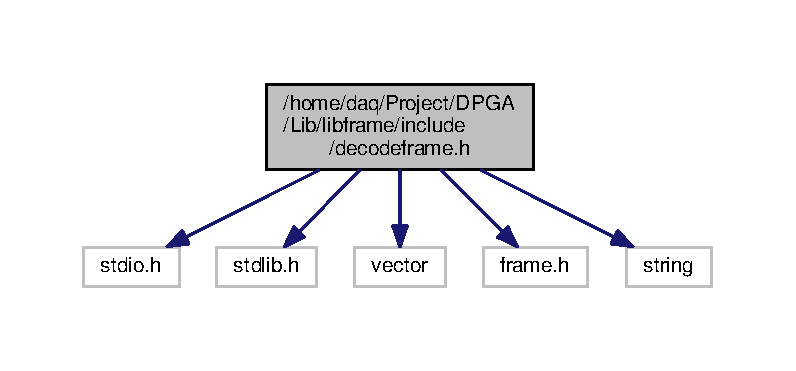
\includegraphics[width=350pt]{decodeframe_8h__incl}
\end{center}
\end{figure}
This graph shows which files directly or indirectly include this file\+:\nopagebreak
\begin{figure}[H]
\begin{center}
\leavevmode
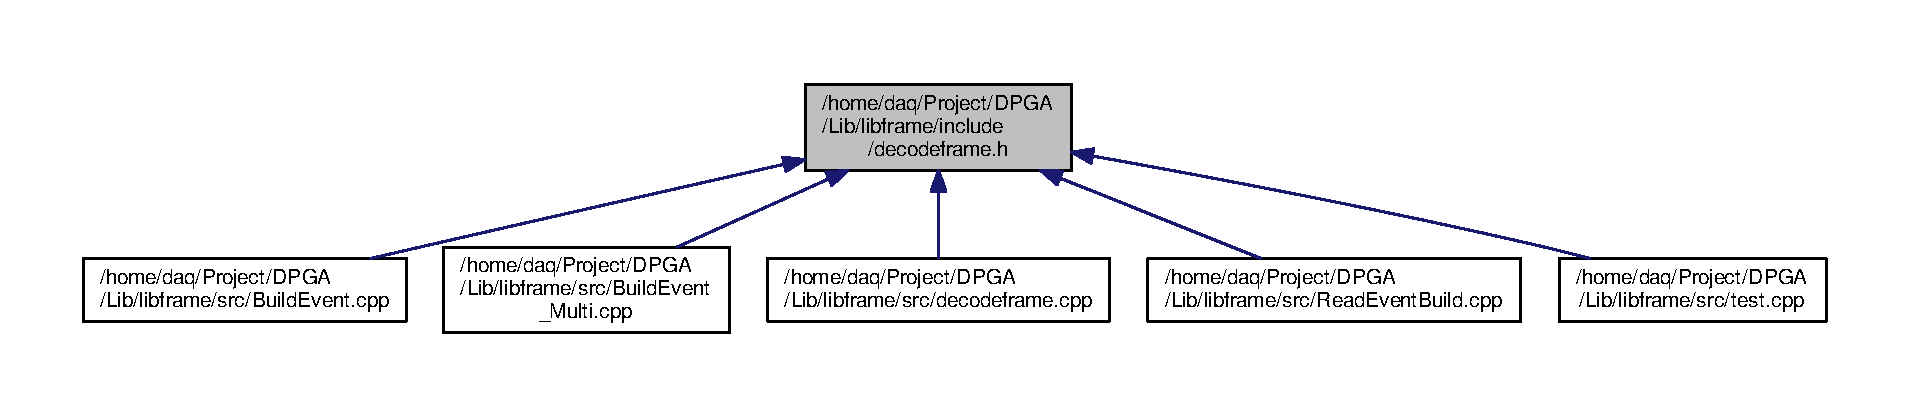
\includegraphics[width=350pt]{decodeframe_8h__dep__incl}
\end{center}
\end{figure}
\subsection*{Classes}
\begin{DoxyCompactItemize}
\item 
struct \hyperlink{structS__ErrorFrame}{S\+\_\+\+Error\+Frame}
\item 
class \hyperlink{classDecodeFrame}{Decode\+Frame}
\end{DoxyCompactItemize}
\subsection*{Macros}
\begin{DoxyCompactItemize}
\item 
\#define \hyperlink{decodeframe_8h_a004a9f800716d02d276a5947ee16bea4}{V\+E\+R\+S\+I\+O\+N\+\_\+\+D\+E\+C\+O\+D\+E\+F\+R\+A\+ME}~\char`\"{}1.\+0.\+0 \char`\"{}
\end{DoxyCompactItemize}
\subsection*{Functions}
\begin{DoxyCompactItemize}
\item 
std\+::string \hyperlink{decodeframe_8h_aaf087ee9fe9aadada3f4d9fa2d913a73}{get\+Version\+Decode\+Frame} ()
\end{DoxyCompactItemize}


\subsection{Detailed Description}
Header Library to decode Frame D\+P\+GA. 

\begin{DoxyAuthor}{Author}
Daniel Lambert 
\end{DoxyAuthor}
\begin{DoxyVersion}{Version}
0.\+1 
\end{DoxyVersion}
\begin{DoxyDate}{Date}
10/207/2017
\end{DoxyDate}
Header Library to decode Frame from thne D\+P\+GA 

\subsection{Macro Definition Documentation}
\mbox{\Hypertarget{decodeframe_8h_a004a9f800716d02d276a5947ee16bea4}\label{decodeframe_8h_a004a9f800716d02d276a5947ee16bea4}} 
\index{decodeframe.\+h@{decodeframe.\+h}!V\+E\+R\+S\+I\+O\+N\+\_\+\+D\+E\+C\+O\+D\+E\+F\+R\+A\+ME@{V\+E\+R\+S\+I\+O\+N\+\_\+\+D\+E\+C\+O\+D\+E\+F\+R\+A\+ME}}
\index{V\+E\+R\+S\+I\+O\+N\+\_\+\+D\+E\+C\+O\+D\+E\+F\+R\+A\+ME@{V\+E\+R\+S\+I\+O\+N\+\_\+\+D\+E\+C\+O\+D\+E\+F\+R\+A\+ME}!decodeframe.\+h@{decodeframe.\+h}}
\subsubsection{\texorpdfstring{V\+E\+R\+S\+I\+O\+N\+\_\+\+D\+E\+C\+O\+D\+E\+F\+R\+A\+ME}{VERSION\_DECODEFRAME}}
{\footnotesize\ttfamily \#define V\+E\+R\+S\+I\+O\+N\+\_\+\+D\+E\+C\+O\+D\+E\+F\+R\+A\+ME~\char`\"{}1.\+0.\+0 \char`\"{}}



\subsection{Function Documentation}
\mbox{\Hypertarget{decodeframe_8h_aaf087ee9fe9aadada3f4d9fa2d913a73}\label{decodeframe_8h_aaf087ee9fe9aadada3f4d9fa2d913a73}} 
\index{decodeframe.\+h@{decodeframe.\+h}!get\+Version\+Decode\+Frame@{get\+Version\+Decode\+Frame}}
\index{get\+Version\+Decode\+Frame@{get\+Version\+Decode\+Frame}!decodeframe.\+h@{decodeframe.\+h}}
\subsubsection{\texorpdfstring{get\+Version\+Decode\+Frame()}{getVersionDecodeFrame()}}
{\footnotesize\ttfamily std\+::string get\+Version\+Decode\+Frame (\begin{DoxyParamCaption}{ }\end{DoxyParamCaption})}


\hypertarget{BuildEvent_8cpp}{}\section{/home/daq/\+Project/\+Firmware\+Tests/\+Serveur\+Udp/libframe/src/\+Build\+Event.cpp File Reference}
\label{BuildEvent_8cpp}\index{/home/daq/\+Project/\+Firmware\+Tests/\+Serveur\+Udp/libframe/src/\+Build\+Event.\+cpp@{/home/daq/\+Project/\+Firmware\+Tests/\+Serveur\+Udp/libframe/src/\+Build\+Event.\+cpp}}
{\ttfamily \#include \char`\"{}decodeframe.\+h\char`\"{}}\newline
{\ttfamily \#include \char`\"{}color.\+h\char`\"{}}\newline
{\ttfamily \#include $<$sstream$>$}\newline
{\ttfamily \#include $<$string$>$}\newline
{\ttfamily \#include $<$stdio.\+h$>$}\newline
{\ttfamily \#include $<$iostream$>$}\newline
{\ttfamily \#include $<$map$>$}\newline
{\ttfamily \#include $<$stdlib.\+h$>$}\newline
{\ttfamily \#include $<$vector$>$}\newline
{\ttfamily \#include $<$string.\+h$>$}\newline
Include dependency graph for Build\+Event.\+cpp\+:\nopagebreak
\begin{figure}[H]
\begin{center}
\leavevmode
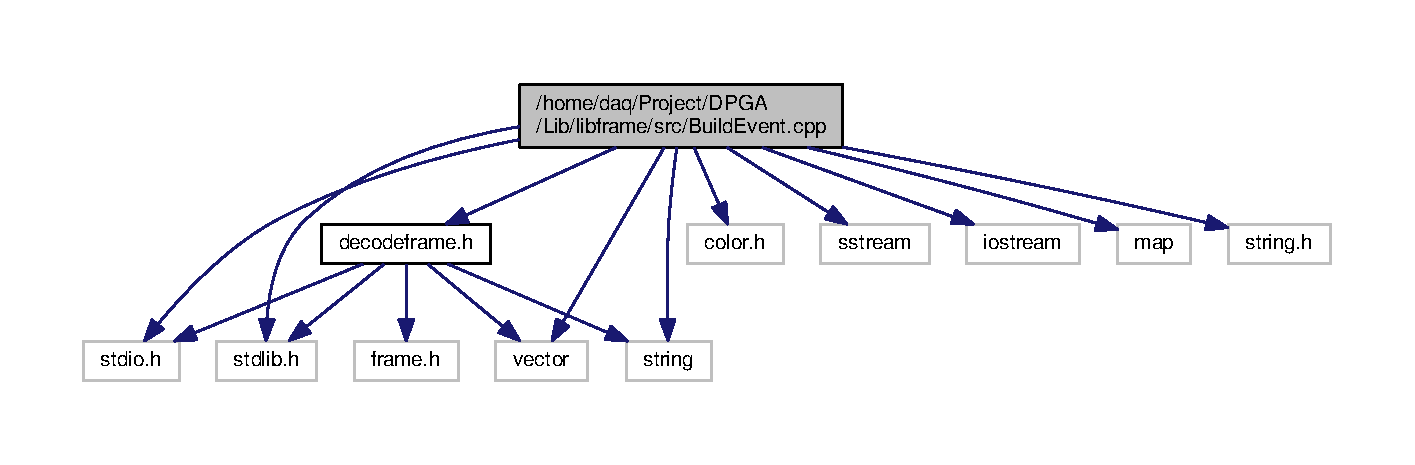
\includegraphics[width=350pt]{BuildEvent_8cpp__incl}
\end{center}
\end{figure}
\subsection*{Functions}
\begin{DoxyCompactItemize}
\item 
const char $\ast$ \hyperlink{BuildEvent_8cpp_a80f947f71feac86fd1d0c826d1e887ea}{Color} (bool c)
\item 
int \hyperlink{BuildEvent_8cpp_ae66f6b31b5ad750f1fe042a706a4e3d4}{main} ()
\end{DoxyCompactItemize}


\subsection{Function Documentation}
\mbox{\Hypertarget{BuildEvent_8cpp_a80f947f71feac86fd1d0c826d1e887ea}\label{BuildEvent_8cpp_a80f947f71feac86fd1d0c826d1e887ea}} 
\index{Build\+Event.\+cpp@{Build\+Event.\+cpp}!Color@{Color}}
\index{Color@{Color}!Build\+Event.\+cpp@{Build\+Event.\+cpp}}
\subsubsection{\texorpdfstring{Color()}{Color()}}
{\footnotesize\ttfamily const char$\ast$ Color (\begin{DoxyParamCaption}\item[{bool}]{c }\end{DoxyParamCaption})}

\mbox{\Hypertarget{BuildEvent_8cpp_ae66f6b31b5ad750f1fe042a706a4e3d4}\label{BuildEvent_8cpp_ae66f6b31b5ad750f1fe042a706a4e3d4}} 
\index{Build\+Event.\+cpp@{Build\+Event.\+cpp}!main@{main}}
\index{main@{main}!Build\+Event.\+cpp@{Build\+Event.\+cpp}}
\subsubsection{\texorpdfstring{main()}{main()}}
{\footnotesize\ttfamily int main (\begin{DoxyParamCaption}{ }\end{DoxyParamCaption})}

6.\+66/1000000

6.\+66

4.\+16/1000000 
\hypertarget{BuildEvent__Multi_8cpp}{}\section{/home/daq/\+Project/\+Firmware\+Tests/\+Serveur\+Udp/libframe/src/\+Build\+Event\+\_\+\+Multi.cpp File Reference}
\label{BuildEvent__Multi_8cpp}\index{/home/daq/\+Project/\+Firmware\+Tests/\+Serveur\+Udp/libframe/src/\+Build\+Event\+\_\+\+Multi.\+cpp@{/home/daq/\+Project/\+Firmware\+Tests/\+Serveur\+Udp/libframe/src/\+Build\+Event\+\_\+\+Multi.\+cpp}}
{\ttfamily \#include \char`\"{}decodeframe.\+h\char`\"{}}\newline
{\ttfamily \#include \char`\"{}color.\+h\char`\"{}}\newline
{\ttfamily \#include $<$sstream$>$}\newline
{\ttfamily \#include $<$string$>$}\newline
{\ttfamily \#include $<$stdio.\+h$>$}\newline
{\ttfamily \#include $<$iostream$>$}\newline
{\ttfamily \#include $<$map$>$}\newline
{\ttfamily \#include $<$stdlib.\+h$>$}\newline
{\ttfamily \#include $<$vector$>$}\newline
{\ttfamily \#include $<$string.\+h$>$}\newline
{\ttfamily \#include $<$dirent.\+h$>$}\newline
{\ttfamily \#include $<$cstring$>$}\newline
{\ttfamily \#include $<$memory$>$}\newline
{\ttfamily \#include $<$sys/types.\+h$>$}\newline
Include dependency graph for Build\+Event\+\_\+\+Multi.\+cpp\+:\nopagebreak
\begin{figure}[H]
\begin{center}
\leavevmode
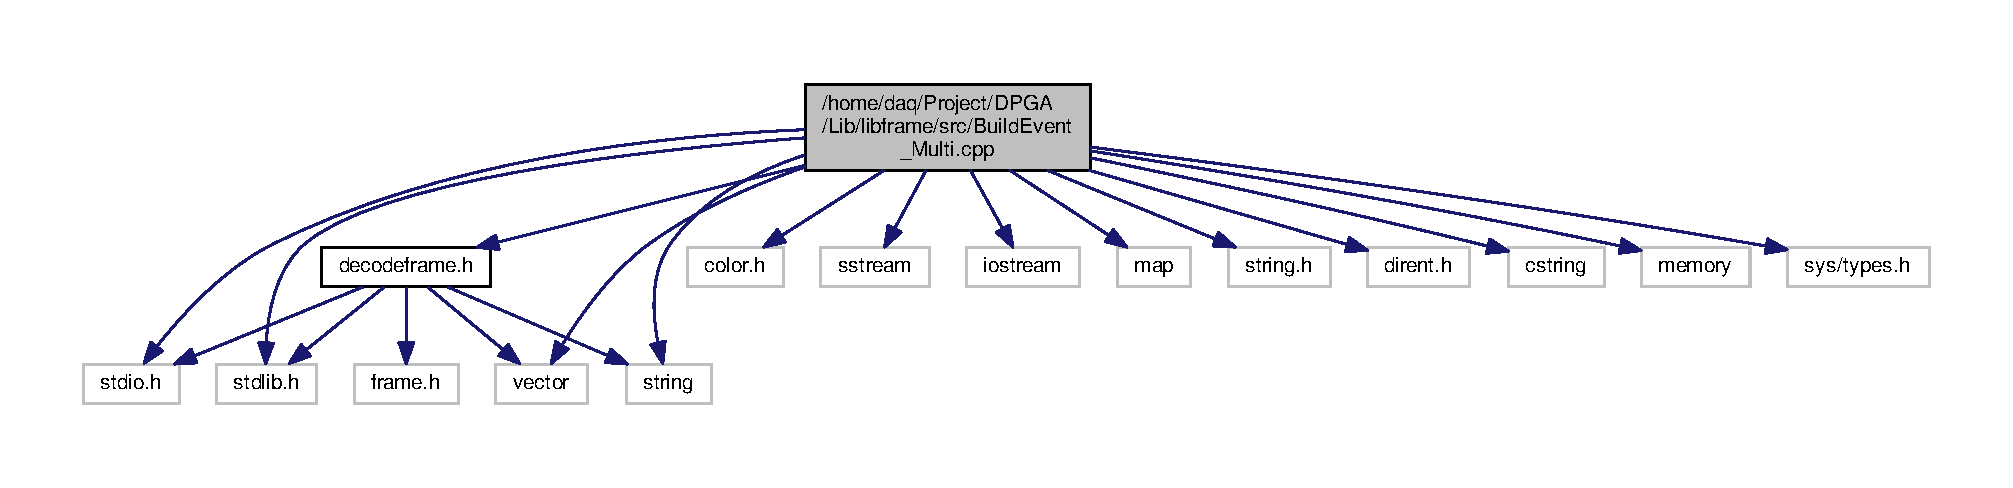
\includegraphics[width=350pt]{BuildEvent__Multi_8cpp__incl}
\end{center}
\end{figure}
\subsection*{Macros}
\begin{DoxyCompactItemize}
\item 
\#define \hyperlink{BuildEvent__Multi_8cpp_a611cc9b5f655508482f3d7a9751c182a}{C\+L\+E\+AR}~\char`\"{}clear\char`\"{}
\end{DoxyCompactItemize}
\subsection*{Functions}
\begin{DoxyCompactItemize}
\item 
const char $\ast$ \hyperlink{BuildEvent__Multi_8cpp_a80f947f71feac86fd1d0c826d1e887ea}{Color} (bool c)
\item 
int \hyperlink{BuildEvent__Multi_8cpp_abf1d945fbac53e8751730aa4cc46d004}{is\+Dir} (char $\ast$s)
\item 
int \hyperlink{BuildEvent__Multi_8cpp_a7f9f7498c35955fe3d8a748182ef77ad}{is\+Dir} (string str, string extension)
\item 
string \hyperlink{BuildEvent__Multi_8cpp_a8b50353dd1f1ca2aeaad7b34716a19e8}{Double\+To\+String} (double var)
\item 
string \hyperlink{BuildEvent__Multi_8cpp_a60970540d743aa7cddcb796855e2b997}{Int\+To\+String} (int var)
\item 
void \hyperlink{BuildEvent__Multi_8cpp_a3f693efd45184c394e10dc61b0023a5b}{Read\+And\+Load\+A\+Directory} (vector$<$ string $>$ \&v\+\_\+\+Complete\+Name\+Of\+File, string Path, string Name\+Of\+Directory, string Extension\+Of\+Research\+File)
\item 
int \hyperlink{BuildEvent__Multi_8cpp_aa586fbfe8f5e5521c969da1c602302a5}{Number\+Of\+Total\+Frame\+For\+Write\+Event\+\_\+\+Pattern} (uint64\+\_\+t Pattern, int Total\+Of\+A\+MS)
\item 
int \hyperlink{BuildEvent__Multi_8cpp_ae66f6b31b5ad750f1fe042a706a4e3d4}{main} ()
\end{DoxyCompactItemize}


\subsection{Detailed Description}
Programme qui construit les event pour la librairie libframe ~\newline
 

montre comment instantier la classe \hyperlink{classDecodeFrame}{Decode\+Frame} avec un fichier ~\newline
 dont le nom /datas1/run0004/\+My\+File\+\_\+eno1@0\+\_\+0.\+bin

Library to decode Frame D\+P\+GA \begin{DoxyAuthor}{Author}
Daniel Lambert \& Arthur Bongrand 
\end{DoxyAuthor}
\begin{DoxyVersion}{Version}
1.\+0 
\end{DoxyVersion}
\begin{DoxyDate}{Date}
21/11/2017
\end{DoxyDate}
Library to decode Frame from the D\+P\+GA 

\subsection{Macro Definition Documentation}
\mbox{\Hypertarget{BuildEvent__Multi_8cpp_a611cc9b5f655508482f3d7a9751c182a}\label{BuildEvent__Multi_8cpp_a611cc9b5f655508482f3d7a9751c182a}} 
\index{Build\+Event\+\_\+\+Multi.\+cpp@{Build\+Event\+\_\+\+Multi.\+cpp}!C\+L\+E\+AR@{C\+L\+E\+AR}}
\index{C\+L\+E\+AR@{C\+L\+E\+AR}!Build\+Event\+\_\+\+Multi.\+cpp@{Build\+Event\+\_\+\+Multi.\+cpp}}
\subsubsection{\texorpdfstring{C\+L\+E\+AR}{CLEAR}}
{\footnotesize\ttfamily \#define C\+L\+E\+AR~\char`\"{}clear\char`\"{}}



\subsection{Function Documentation}
\mbox{\Hypertarget{BuildEvent__Multi_8cpp_a80f947f71feac86fd1d0c826d1e887ea}\label{BuildEvent__Multi_8cpp_a80f947f71feac86fd1d0c826d1e887ea}} 
\index{Build\+Event\+\_\+\+Multi.\+cpp@{Build\+Event\+\_\+\+Multi.\+cpp}!Color@{Color}}
\index{Color@{Color}!Build\+Event\+\_\+\+Multi.\+cpp@{Build\+Event\+\_\+\+Multi.\+cpp}}
\subsubsection{\texorpdfstring{Color()}{Color()}}
{\footnotesize\ttfamily const char$\ast$ Color (\begin{DoxyParamCaption}\item[{bool}]{c }\end{DoxyParamCaption})}

\mbox{\Hypertarget{BuildEvent__Multi_8cpp_a8b50353dd1f1ca2aeaad7b34716a19e8}\label{BuildEvent__Multi_8cpp_a8b50353dd1f1ca2aeaad7b34716a19e8}} 
\index{Build\+Event\+\_\+\+Multi.\+cpp@{Build\+Event\+\_\+\+Multi.\+cpp}!Double\+To\+String@{Double\+To\+String}}
\index{Double\+To\+String@{Double\+To\+String}!Build\+Event\+\_\+\+Multi.\+cpp@{Build\+Event\+\_\+\+Multi.\+cpp}}
\subsubsection{\texorpdfstring{Double\+To\+String()}{DoubleToString()}}
{\footnotesize\ttfamily string Double\+To\+String (\begin{DoxyParamCaption}\item[{double}]{var }\end{DoxyParamCaption})}

\mbox{\Hypertarget{BuildEvent__Multi_8cpp_a60970540d743aa7cddcb796855e2b997}\label{BuildEvent__Multi_8cpp_a60970540d743aa7cddcb796855e2b997}} 
\index{Build\+Event\+\_\+\+Multi.\+cpp@{Build\+Event\+\_\+\+Multi.\+cpp}!Int\+To\+String@{Int\+To\+String}}
\index{Int\+To\+String@{Int\+To\+String}!Build\+Event\+\_\+\+Multi.\+cpp@{Build\+Event\+\_\+\+Multi.\+cpp}}
\subsubsection{\texorpdfstring{Int\+To\+String()}{IntToString()}}
{\footnotesize\ttfamily string Int\+To\+String (\begin{DoxyParamCaption}\item[{int}]{var }\end{DoxyParamCaption})}

\mbox{\Hypertarget{BuildEvent__Multi_8cpp_abf1d945fbac53e8751730aa4cc46d004}\label{BuildEvent__Multi_8cpp_abf1d945fbac53e8751730aa4cc46d004}} 
\index{Build\+Event\+\_\+\+Multi.\+cpp@{Build\+Event\+\_\+\+Multi.\+cpp}!is\+Dir@{is\+Dir}}
\index{is\+Dir@{is\+Dir}!Build\+Event\+\_\+\+Multi.\+cpp@{Build\+Event\+\_\+\+Multi.\+cpp}}
\subsubsection{\texorpdfstring{is\+Dir()}{isDir()}\hspace{0.1cm}{\footnotesize\ttfamily [1/2]}}
{\footnotesize\ttfamily int is\+Dir (\begin{DoxyParamCaption}\item[{char $\ast$}]{s }\end{DoxyParamCaption})}

\mbox{\Hypertarget{BuildEvent__Multi_8cpp_a7f9f7498c35955fe3d8a748182ef77ad}\label{BuildEvent__Multi_8cpp_a7f9f7498c35955fe3d8a748182ef77ad}} 
\index{Build\+Event\+\_\+\+Multi.\+cpp@{Build\+Event\+\_\+\+Multi.\+cpp}!is\+Dir@{is\+Dir}}
\index{is\+Dir@{is\+Dir}!Build\+Event\+\_\+\+Multi.\+cpp@{Build\+Event\+\_\+\+Multi.\+cpp}}
\subsubsection{\texorpdfstring{is\+Dir()}{isDir()}\hspace{0.1cm}{\footnotesize\ttfamily [2/2]}}
{\footnotesize\ttfamily int is\+Dir (\begin{DoxyParamCaption}\item[{string}]{str,  }\item[{string}]{extension }\end{DoxyParamCaption})}

\mbox{\Hypertarget{BuildEvent__Multi_8cpp_ae66f6b31b5ad750f1fe042a706a4e3d4}\label{BuildEvent__Multi_8cpp_ae66f6b31b5ad750f1fe042a706a4e3d4}} 
\index{Build\+Event\+\_\+\+Multi.\+cpp@{Build\+Event\+\_\+\+Multi.\+cpp}!main@{main}}
\index{main@{main}!Build\+Event\+\_\+\+Multi.\+cpp@{Build\+Event\+\_\+\+Multi.\+cpp}}
\subsubsection{\texorpdfstring{main()}{main()}}
{\footnotesize\ttfamily int main (\begin{DoxyParamCaption}{ }\end{DoxyParamCaption})}

6.\+66/1000000

6.\+66

4.\+16/1000000 \mbox{\Hypertarget{BuildEvent__Multi_8cpp_aa586fbfe8f5e5521c969da1c602302a5}\label{BuildEvent__Multi_8cpp_aa586fbfe8f5e5521c969da1c602302a5}} 
\index{Build\+Event\+\_\+\+Multi.\+cpp@{Build\+Event\+\_\+\+Multi.\+cpp}!Number\+Of\+Total\+Frame\+For\+Write\+Event\+\_\+\+Pattern@{Number\+Of\+Total\+Frame\+For\+Write\+Event\+\_\+\+Pattern}}
\index{Number\+Of\+Total\+Frame\+For\+Write\+Event\+\_\+\+Pattern@{Number\+Of\+Total\+Frame\+For\+Write\+Event\+\_\+\+Pattern}!Build\+Event\+\_\+\+Multi.\+cpp@{Build\+Event\+\_\+\+Multi.\+cpp}}
\subsubsection{\texorpdfstring{Number\+Of\+Total\+Frame\+For\+Write\+Event\+\_\+\+Pattern()}{NumberOfTotalFrameForWriteEvent\_Pattern()}}
{\footnotesize\ttfamily int Number\+Of\+Total\+Frame\+For\+Write\+Event\+\_\+\+Pattern (\begin{DoxyParamCaption}\item[{uint64\+\_\+t}]{Pattern,  }\item[{int}]{Total\+Of\+A\+MS }\end{DoxyParamCaption})}

\mbox{\Hypertarget{BuildEvent__Multi_8cpp_a3f693efd45184c394e10dc61b0023a5b}\label{BuildEvent__Multi_8cpp_a3f693efd45184c394e10dc61b0023a5b}} 
\index{Build\+Event\+\_\+\+Multi.\+cpp@{Build\+Event\+\_\+\+Multi.\+cpp}!Read\+And\+Load\+A\+Directory@{Read\+And\+Load\+A\+Directory}}
\index{Read\+And\+Load\+A\+Directory@{Read\+And\+Load\+A\+Directory}!Build\+Event\+\_\+\+Multi.\+cpp@{Build\+Event\+\_\+\+Multi.\+cpp}}
\subsubsection{\texorpdfstring{Read\+And\+Load\+A\+Directory()}{ReadAndLoadADirectory()}}
{\footnotesize\ttfamily void Read\+And\+Load\+A\+Directory (\begin{DoxyParamCaption}\item[{vector$<$ string $>$ \&}]{v\+\_\+\+Complete\+Name\+Of\+File,  }\item[{string}]{Path,  }\item[{string}]{Name\+Of\+Directory,  }\item[{string}]{Extension\+Of\+Research\+File }\end{DoxyParamCaption})}


\hypertarget{decodeframe_8cpp}{}\section{/home/daq/\+Project/\+Firmware\+Tests/\+Serveur\+Udp/libframe/src/decodeframe.cpp File Reference}
\label{decodeframe_8cpp}\index{/home/daq/\+Project/\+Firmware\+Tests/\+Serveur\+Udp/libframe/src/decodeframe.\+cpp@{/home/daq/\+Project/\+Firmware\+Tests/\+Serveur\+Udp/libframe/src/decodeframe.\+cpp}}
{\ttfamily \#include $<$string.\+h$>$}\newline
{\ttfamily \#include $<$assert.\+h$>$}\newline
{\ttfamily \#include \char`\"{}decodeframe.\+h\char`\"{}}\newline
Include dependency graph for decodeframe.\+cpp\+:\nopagebreak
\begin{figure}[H]
\begin{center}
\leavevmode
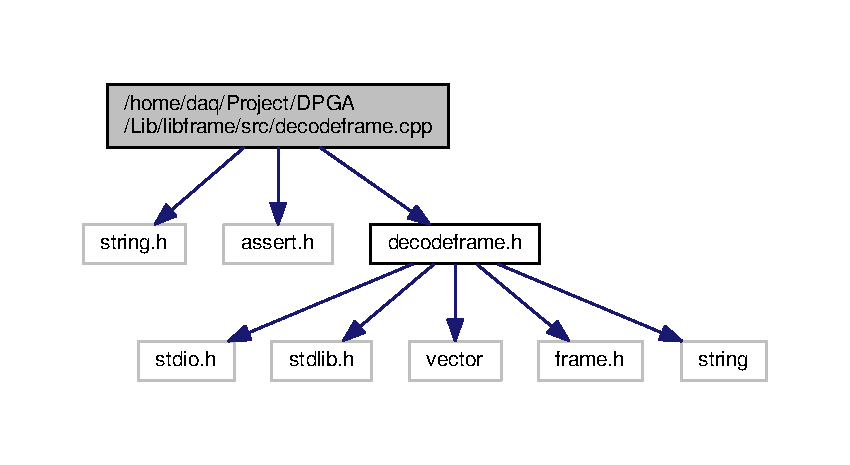
\includegraphics[width=350pt]{decodeframe_8cpp__incl}
\end{center}
\end{figure}
\subsection*{Macros}
\begin{DoxyCompactItemize}
\item 
\#define \hyperlink{decodeframe_8cpp_a3848879e2e2db405665a8ada190ddcd8}{D\+E\+C\+S\+OC}(a)~((a \& 0xff00) $>$$>$ 8)
\end{DoxyCompactItemize}
\subsection*{Functions}
\begin{DoxyCompactItemize}
\item 
std\+::string \hyperlink{decodeframe_8cpp_aaf087ee9fe9aadada3f4d9fa2d913a73}{get\+Version\+Decode\+Frame} ()
\end{DoxyCompactItemize}


\subsection{Detailed Description}
Programme qui construit les event pour la librairie libframe ~\newline
 

Library to decode Frame D\+P\+GA.

montre comment instantier la classe \hyperlink{classDecodeFrame}{Decode\+Frame} avec un fichier ~\newline
 dont le nom /datas1/run0004/\+My\+File\+\_\+eno1@0\+\_\+0.\+bin

Library to decode Frame D\+P\+GA \begin{DoxyAuthor}{Author}
Daniel Lambert \& Arthur Bongrand 
\end{DoxyAuthor}
\begin{DoxyVersion}{Version}
1.\+0 
\end{DoxyVersion}
\begin{DoxyDate}{Date}
21/11/2017
\end{DoxyDate}
Library to decode Frame from the D\+P\+GA

\begin{DoxyAuthor}{Author}
Daniel Lambert 
\end{DoxyAuthor}
\begin{DoxyVersion}{Version}
0.\+1 
\end{DoxyVersion}
\begin{DoxyDate}{Date}
10/207/2017
\end{DoxyDate}
Library to decode Frame from the D\+P\+GA 

\subsection{Macro Definition Documentation}
\mbox{\Hypertarget{decodeframe_8cpp_a3848879e2e2db405665a8ada190ddcd8}\label{decodeframe_8cpp_a3848879e2e2db405665a8ada190ddcd8}} 
\index{decodeframe.\+cpp@{decodeframe.\+cpp}!D\+E\+C\+S\+OC@{D\+E\+C\+S\+OC}}
\index{D\+E\+C\+S\+OC@{D\+E\+C\+S\+OC}!decodeframe.\+cpp@{decodeframe.\+cpp}}
\subsubsection{\texorpdfstring{D\+E\+C\+S\+OC}{DECSOC}}
{\footnotesize\ttfamily \#define D\+E\+C\+S\+OC(\begin{DoxyParamCaption}\item[{}]{a }\end{DoxyParamCaption})~((a \& 0xff00) $>$$>$ 8)}



\subsection{Function Documentation}
\mbox{\Hypertarget{decodeframe_8cpp_aaf087ee9fe9aadada3f4d9fa2d913a73}\label{decodeframe_8cpp_aaf087ee9fe9aadada3f4d9fa2d913a73}} 
\index{decodeframe.\+cpp@{decodeframe.\+cpp}!get\+Version\+Decode\+Frame@{get\+Version\+Decode\+Frame}}
\index{get\+Version\+Decode\+Frame@{get\+Version\+Decode\+Frame}!decodeframe.\+cpp@{decodeframe.\+cpp}}
\subsubsection{\texorpdfstring{get\+Version\+Decode\+Frame()}{getVersionDecodeFrame()}}
{\footnotesize\ttfamily std\+::string get\+Version\+Decode\+Frame (\begin{DoxyParamCaption}{ }\end{DoxyParamCaption})}


\hypertarget{ReadEventBuild_8cpp}{}\section{/home/daq/\+Project/\+D\+P\+G\+A/\+Lib/libframe/src/\+Read\+Event\+Build.cpp File Reference}
\label{ReadEventBuild_8cpp}\index{/home/daq/\+Project/\+D\+P\+G\+A/\+Lib/libframe/src/\+Read\+Event\+Build.\+cpp@{/home/daq/\+Project/\+D\+P\+G\+A/\+Lib/libframe/src/\+Read\+Event\+Build.\+cpp}}
{\ttfamily \#include \char`\"{}decodeframe.\+h\char`\"{}}\newline
{\ttfamily \#include \char`\"{}color.\+h\char`\"{}}\newline
{\ttfamily \#include $<$sstream$>$}\newline
{\ttfamily \#include $<$string$>$}\newline
{\ttfamily \#include $<$stdio.\+h$>$}\newline
{\ttfamily \#include $<$iostream$>$}\newline
{\ttfamily \#include $<$map$>$}\newline
{\ttfamily \#include $<$stdlib.\+h$>$}\newline
{\ttfamily \#include $<$vector$>$}\newline
{\ttfamily \#include $<$string.\+h$>$}\newline
Include dependency graph for Read\+Event\+Build.\+cpp\+:\nopagebreak
\begin{figure}[H]
\begin{center}
\leavevmode
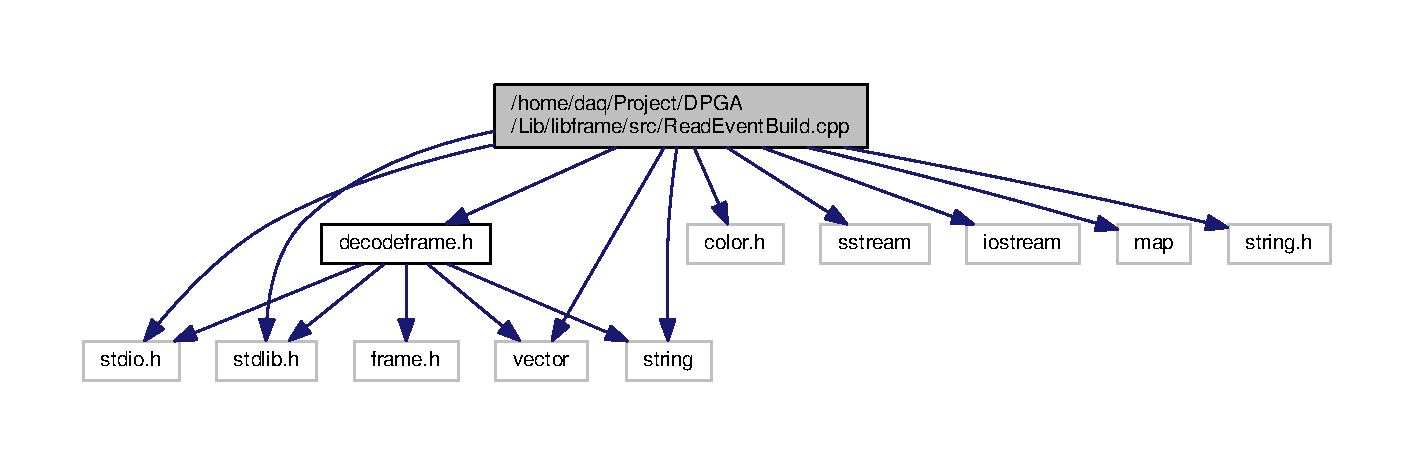
\includegraphics[width=350pt]{ReadEventBuild_8cpp__incl}
\end{center}
\end{figure}
\subsection*{Functions}
\begin{DoxyCompactItemize}
\item 
const char $\ast$ \hyperlink{ReadEventBuild_8cpp_a80f947f71feac86fd1d0c826d1e887ea}{Color} (bool c)
\item 
int \hyperlink{ReadEventBuild_8cpp_ae66f6b31b5ad750f1fe042a706a4e3d4}{main} ()
\end{DoxyCompactItemize}


\subsection{Function Documentation}
\mbox{\Hypertarget{ReadEventBuild_8cpp_a80f947f71feac86fd1d0c826d1e887ea}\label{ReadEventBuild_8cpp_a80f947f71feac86fd1d0c826d1e887ea}} 
\index{Read\+Event\+Build.\+cpp@{Read\+Event\+Build.\+cpp}!Color@{Color}}
\index{Color@{Color}!Read\+Event\+Build.\+cpp@{Read\+Event\+Build.\+cpp}}
\subsubsection{\texorpdfstring{Color()}{Color()}}
{\footnotesize\ttfamily const char$\ast$ Color (\begin{DoxyParamCaption}\item[{bool}]{c }\end{DoxyParamCaption})}

\mbox{\Hypertarget{ReadEventBuild_8cpp_ae66f6b31b5ad750f1fe042a706a4e3d4}\label{ReadEventBuild_8cpp_ae66f6b31b5ad750f1fe042a706a4e3d4}} 
\index{Read\+Event\+Build.\+cpp@{Read\+Event\+Build.\+cpp}!main@{main}}
\index{main@{main}!Read\+Event\+Build.\+cpp@{Read\+Event\+Build.\+cpp}}
\subsubsection{\texorpdfstring{main()}{main()}}
{\footnotesize\ttfamily int main (\begin{DoxyParamCaption}{ }\end{DoxyParamCaption})}

6.\+66/1000000

6.\+66

4.\+16/1000000 
\hypertarget{test_8cpp}{}\section{/home/daq/\+Project/\+Firmware\+Tests/\+Serveur\+Udp/libframe/src/test.cpp File Reference}
\label{test_8cpp}\index{/home/daq/\+Project/\+Firmware\+Tests/\+Serveur\+Udp/libframe/src/test.\+cpp@{/home/daq/\+Project/\+Firmware\+Tests/\+Serveur\+Udp/libframe/src/test.\+cpp}}
{\ttfamily \#include \char`\"{}decodeframe.\+h\char`\"{}}\newline
{\ttfamily \#include \char`\"{}color.\+h\char`\"{}}\newline
{\ttfamily \#include $<$sstream$>$}\newline
{\ttfamily \#include $<$string$>$}\newline
{\ttfamily \#include $<$stdio.\+h$>$}\newline
{\ttfamily \#include $<$iostream$>$}\newline
{\ttfamily \#include $<$map$>$}\newline
{\ttfamily \#include $<$stdlib.\+h$>$}\newline
{\ttfamily \#include $<$vector$>$}\newline
Include dependency graph for test.\+cpp\+:\nopagebreak
\begin{figure}[H]
\begin{center}
\leavevmode
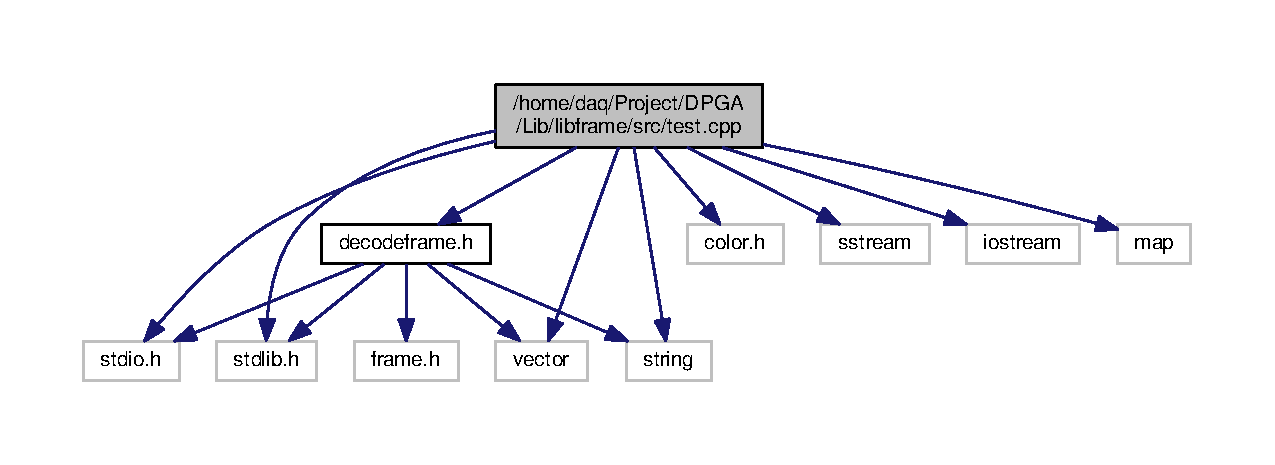
\includegraphics[width=350pt]{test_8cpp__incl}
\end{center}
\end{figure}
\subsection*{Functions}
\begin{DoxyCompactItemize}
\item 
const char $\ast$ \hyperlink{test_8cpp_a80f947f71feac86fd1d0c826d1e887ea}{Color} (bool c)
\item 
int \hyperlink{test_8cpp_ae66f6b31b5ad750f1fe042a706a4e3d4}{main} ()
\end{DoxyCompactItemize}


\subsection{Function Documentation}
\mbox{\Hypertarget{test_8cpp_a80f947f71feac86fd1d0c826d1e887ea}\label{test_8cpp_a80f947f71feac86fd1d0c826d1e887ea}} 
\index{test.\+cpp@{test.\+cpp}!Color@{Color}}
\index{Color@{Color}!test.\+cpp@{test.\+cpp}}
\subsubsection{\texorpdfstring{Color()}{Color()}}
{\footnotesize\ttfamily const char$\ast$ Color (\begin{DoxyParamCaption}\item[{bool}]{c }\end{DoxyParamCaption})}

\mbox{\Hypertarget{test_8cpp_ae66f6b31b5ad750f1fe042a706a4e3d4}\label{test_8cpp_ae66f6b31b5ad750f1fe042a706a4e3d4}} 
\index{test.\+cpp@{test.\+cpp}!main@{main}}
\index{main@{main}!test.\+cpp@{test.\+cpp}}
\subsubsection{\texorpdfstring{main()}{main()}}
{\footnotesize\ttfamily int main (\begin{DoxyParamCaption}{ }\end{DoxyParamCaption})}


%--- End generated contents ---

% Index
\backmatter
\newpage
\phantomsection
\clearemptydoublepage
\addcontentsline{toc}{chapter}{Index}
\printindex

\end{document}
